\documentclass[10pt]{extbook}
\usepackage[T1]{fontenc}
\usepackage[utf8]{inputenc}
\usepackage[document]{ragged2e}
\usepackage{microtype}
\usepackage{mlmodern}
%\usepackage[bitstream-charter]{mathdesign}
%\usepackage{scholax}
%\usepackage{XCharter}
%\usepackage{CharisSIL}
%\usepackage[usefilenames,RMstyle={Text, Text},SSstyle={Text,Bold},TTstyle={Text,Semibold},DefaultFeatures={Ligatures=Common}]{plex-otf} %
%\usepackage[p]{scholax}
\usepackage[default,regular,bold]{sourceserifpro}
\usepackage[all]{nowidow}
\usepackage{graphicx}
\usepackage{svg}
\usepackage[pdfa]{hyperref}
\usepackage{color}
\usepackage{makecell}
\usepackage{setspace}
\usepackage{parskip}
\usepackage[a4paper, inner=4.0cm, outer=5.2cm]{geometry}
\usepackage{listings}
\definecolor{dkgreen}{rgb}{0.1,0.5,0.1}
\definecolor{greengray}{rgb}{0.517,0.761,0.404}
\definecolor{orange}{rgb}{0.717,0.274,0.105}
\definecolor{blue}{rgb}{0.164,0.317,0.600}
\definecolor{background}{rgb}{0.990,0.990,0.990}
\lstset {
    frame=lrtb,
	language=java,
	aboveskip=0.7cm,
	belowskip=0.2cm,
	showstringspaces=false,
	columns=flexible,
	basicstyle={\small\ttfamily},
	numbers=none,
	backgroundcolor=\color{background},
	numberstyle=\tiny\color{dkgreen},
	keywordstyle=\color{blue},
	commentstyle=\color{greengray},
	stringstyle=\color{orange},
	breaklines=true,
	breakatwhitespace=true,
	tabsize=3
}

\newtheorem{thm}{Teorema}
\setlength{\tabcolsep}{0.5em} % for the horizontal padding
{\renewcommand{\arraystretch}{1.35}% for the vertical padding

\usepackage{fancyhdr}


\pagestyle{fancy}
\fancyhf{}
\fancyhead[LE,RO]{\leftmark}
\fancyfoot[LE,RO]{\thepage}

\renewcommand{\headrulewidth}{1pt}
%\renewcommand{\footrulewidth}{1pt}

\usepackage{titlesec}

\begin{document}
%\setmonofont[Scale=.93]{IBM Plex Mono Medium}


\begin{titlepage}
        \begin{center}
                \Large
                \textbf{UNIVERSITÀ DEGLI STUDI DI TRIESTE}

                \par\noindent\rule{\textwidth}{0.8pt}
                \vspace*{0.6cm}

                \large
                \emph{Marco Sgobino}

                \large
                \vspace*{0.6cm}

                \Large Notes from the course of
                \vspace*{0.6cm}

                \Huge
                \textsc{Computer Networks II and Introduction to Cybersecurity}
                \vspace*{.1cm}

                %\large 
                %\emph{sezione intermedia}

                \vspace*{2cm}

                \begin{center}
                        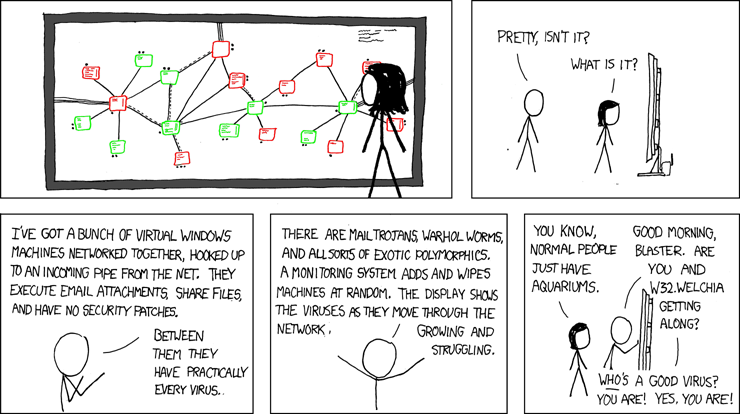
\includegraphics[width=.9\textwidth, keepaspectratio]{./pics/networks-titlepage.png}
                \end{center}

                \vfill

                \par\noindent\rule{\textwidth}{0.8pt}
                \vspace*{0.6cm}
                \large
                \emph{Academic Year 2021-2022}

        \end{center}
\end{titlepage}


\setstretch{1.25}
\setlength{\headsep}{30pt}
\setlength{\footskip}{40pt}
\setlength{\marginparsep}{20pt}
\setlength{\marginparwidth}{50pt}
%\title{Computer Networks 2 and Introduction to Cybersecurity}
%\author{Marco Sgobino}
%\maketitle
\tableofcontents

\setsansfont{Source Serif 4 Display}

\titleformat{\part}[display]
{\Huge\bfseries\sffamily}{}{0pt}{\center{ Part \thepart\ \ \\ \ \ }}
\titleformat{\chapter}[display]
{\Huge\bfseries\sffamily}{}{0pt}{Chapter \thechapter\\\bigskip}
\titleformat{\section}[display]
{\LARGE\bfseries\sffamily}{}{0pt}{\thesection\ \ \ \ \ }
\titleformat{\subsection}[display]
{\Large\bfseries\sffamily}{}{0pt}{\thesubsection\ \ \ \ \ }
\titleformat{\subsubsection}[display]
{\large\bfseries\sffamily}{}{0pt}{}

\part{Security in Networking Protocols}

\chapter{Transmission Control Protocol internals}

\section{TCP Basis}

\subsection{Recap}

TCP is a protocol that has the following remarkable properties,

\begin{enumerate}
	\item it is \emph{connection-oriented}: before transmitting data, a
		connection must be established \--- this is different to what
		IP protocol does in network layer, since in IP protocol there
        lies no concept of connection, and messages are exchanged under the
        paradigm of \emph{packet switching}\footnote{In telecommunications,
        packet switching is a method of grouping data into packets that are
    transmitted over a digital network. Packets are made of a header and a
payload. Data in the header is used by networking hardware to direct the packet
to its destination, where the payload is extracted and used by an operating
system, application software, or higher layer protocols. Packet switching is
the primary basis for data communications in computer networks worldwide. };
	\item it is \emph{reliable}: it assures all segments are correctly
		delivered through use of \emph{ACK} mechanism, and \textbf{at
		most once} \--- again, this is different to IP layer, since IP
        packets are just sent one after the other, unreliably, and there is no
        guarantee that they will be delivered, let alone in their correct
        ordering;
	\item it offers a \emph{sliding window} mechanism for congestion control
		and stream control. This assures read and send buffers are
		well-optimized in both sender and receiver \--- this feature is
		much important since it allows fine-tuning the connection and
		avoiding waste of resources;
	\item it is \emph{byte-oriented}: the byte stream is fragmented into
		multiple segments, and composed again after getting to
		destination \--- in this manner, huge payloads can be reliably
		delivered in multiple segments, each one having the correct
		order to the application. Application has the necessary information
		to easily reconstruct the correct ordering of the acquired 
		information.
\end{enumerate}

Ultimately, TCP allows creating connections between application processes,
offering multiple services to the upper layers. Connections are possible thanks
to the four above characteristics of the TCP layer.

\subsubsection{Sockets}

The TCP makes use of \emph{sockets} abstraction as a way of serving data to the
above application layer. The logical structure is the following one: there are
two entities, the client and the server. The client first authenticates to the
server; the server then opens a connection and the client executes the
subsequent send-receive loop. Both server and client need to create a
\emph{socket} $s$ (a UNIX-like file abstraction), that can be used to send and
receive data. Client connect $s$ to \texttt{IP-srv}, \texttt{port-srv}, while
the server operates a similar procedure on its own sockets. Each socket is then
bound to a specific IP address and a specific \emph{port number}, according to
the just-created connection specifics.

The communication takes place on $s$ by means of an application protocol, with
applications exchanging data each other. The connection is said to be
\emph{reliable}: losses and packet loss are carefully managed by the TCP
protocol, and segments\footnote{\emph{Segments} refer to the particular kind of
package that TCP protocol exchange. Usually, in literature one could find the
term package referring to TCP segments; while this is not fully correct, it may
be acceptable when there is no ambiguity.} are collected in the very same order
as they are sent.

A very simplified pseudo-code at client's side for TCP is as follows,

\begin{verbatim} int s; s := socket(...); 
connect(s, IP-srv, port-srv,...); 
...
send (s, msgl, ...); 
... 
msg2 := receive(s,...); 
... 
\end{verbatim}

where the notation \emph{...} denotes possibly code in between two
instructions. In the above code, a client wants to send data to a remove server
having a specific IP address and a port number. The client first creates a
socket, then connects it to the server IP address and to the corresponding port
number. After connection has been established, the client can subsequently
invoke \texttt{send()} to command TCP layer to deliver desired data to the
other end. To the very same socket, data can be received as well: by invoking
\texttt{receive()} the client can successfully retrieve eventual data sent by
the server. Socket acts as an \emph{abstraction} for the application layer, for
which a socket can be simply thought as a \textbf{data sink} or \textbf{data
source}.

At server side, the logical structure is quite different. A server creates
a socket \texttt{s1}, chooses a port number to bind to that socket (usually a
standard one), then it declares \emph{willingness to accept connections} on
\texttt{s1}, and finally it awaits for connection requests on \texttt{s1}. Upon
receiving a connection request, the server handles it by creating
\emph{another} socket \texttt{s2} and managing the connection on this newly
generated socket, this time with a different port number. 

Basically, it creates two different sockets: the first is kept alive to accept
new connections, and the second one is created on-demand, and it is required to
actually manage the connection. A \emph{different} socket is required for each
connection. A server usually remains on \emph{sleep} until a connection is
requested, awaiting a request on the main socket.

\begin{verbatim} 
s1 := socket(...);
bind(s1, portsrvm ...);
listen(s1,...);
s2 := accept(s1,...); // another socket
... 
msg1 := receive(s2,...);
...
send(s2,msg2,...);
... 
\end{verbatim}

Details of the above code largely depend on the platform on which the server is
operating.

\subsection{TCP Implementation}

TCP layer is built \emph{on top} of the IP layer. Since there are many differences
between TCP and IP, set aside their abstraction layer, TCP should be properly
built to manage IP differences and quirks. 

IP protocol operates between \emph{nodes}: it is \emph{connectionless},
\textbf{unreliable}, and is \emph{message-oriented}. The \textbf{Maximum
Transmission Unit} size of an IP packet is $MTU = 64KB$: this implicitly means
a TCP segment can never be greater than the MTU, because a TCP segment is
carried \emph{inside} an IP packet.

In TCP, communication happens to be \textbf{bidirectional}, with a pattern that
depends on the application protocol. The send\----receive patterns heavily depends
on the application itself \-- browser-related send\----receive sequences are
very different from, let's say, an e-mail client send\----receive sequence.
There is no guarantee that two different application protocols will exchange a
similar amount and kind of TCP messages, let alone the very same ones.

As already mentioned, TCP layers communicate between themselves in terms of
\emph{segments}. A segment is a single \emph{message between TCP layers}, and
contains a \emph{TCP header} and \--- eventually \--- data, that is said to be
\emph{payload}. The difference between information in header and information in
payload is that the first one is strictly required by the TCP layer, while the
second one is information required by the application layer. The latter may be
absent in some segments.

Payload in fact can either be $0$ bytes long or carry some information (wanted
by the application layer). \emph{A TCP segment must be small enough to fit in a
single IP packet}, hence IP header and TCP segment size should be no greater
than $64KB$, the MTU of an IP packet.

Since a packet is composed by a IP header, whose payload is a TCP segment, and the
TCP segment is in turn composed by a TCP header, followed by eventual
application data, the shape of a packet plus its segment can be summarized as
follows,

\begin{verbatim}
| IP header | TCP header |  Payload ***  |
\end{verbatim}

Usually, IP header size is usually $20$ bytes, as well as TCP
header that is $20$ bytes. The IP datagram can be greater up to $64KB$, with
the first $40$ to $50$ bytes reserved to headers. Thus,

\begin{verbatim}
| IP header | TCP header |  Payload ***  |
   20 byte     20 byte        greater
\end{verbatim}

Segments can carry portions of the original data. For instance, in a video
stream many, many segments should be sent to client in order to carry enough
information and let application layer reconstruct the video correctly. For
this reason, in application layer, one huge application message could correspond to
\emph{many segments} in TCP layer, in \textbf{both} directions. At TCP
level multiple segments are usually required in order to send a single
`big' application-level message.

Basically, this means that while for the application layer a single
\texttt{send()} may suffice to send an entire file or all the information
required, from the TCP layer's point of view many and many segments may be
required, typically many more than the number of \texttt{send()} commands
invoked by the application (at least, an number of them equal to the
\texttt{send()} invocation should be sent).

\subsubsection{The connection state}

TCP takes care of creating \emph{connections} between processes. There would be
no actual TCP data exchange without an established connection. Connections do
possess their own \emph{state}, which fundamentally and univocally describes a
connection. It is enough to represent each connection with their \texttt{<id>}
and \texttt{<state>}, with the \texttt{<id>} field that contains essentially
$4$ informations,
\begin{enumerate}
    \item the \texttt{local IP} address;
    \item the \texttt{local port} number;
    \item the \texttt{remote IP} address;
    \item the \texttt{remote port} number.
\end{enumerate}

Four and only four informations are required: the IP address and the
port number of each connection's endpoint.

Each connection is then associated to a \texttt{state}, that serves as a
description of the actual state in which the connection lies. The state of the
connection describes precisely the condition in which the connection lies (is
it running? is it closed?).

Information regarding a TCP connection must reside in the packet and in the segment
header, so each received segment can be sorted out and managed properly. IP
addresses are extracted from the IP header, while port numbers are extracted
from TCP header, thus it suffices to look at the IP packet plus the TCP header.

Information in header is not sufficient: each endpoint must keep track of the
connection with a \emph{state variable}. The connection <state> includes
information on the \textbf{Maximum Segment Size} (MSS), which is the maximum
size of the \emph{data part} of a segment that the other part is willing to
receive. The MSS is negotiated upon connection opening \--- this value is, in
practice, identical in both direction and \textbf{not arbitrary}. In most
cases and for historical reasons, there are only $2$ possible values that
depend whether the connection:

\begin{itemize}
    \item \emph{lies on different networks} (connection through internet), MSS
        is $536$ bytes (MTU=576), that is the maximum segment size that can fit
        in the smallest possible packet \-- historically this was the most
        reliable option;
    \item \emph{lies on the same network} (connection through ethernet), MSS is
        $1460$ bytes (MTU=1500), which corresponds to ethernet MTU minus the IP
        header and TCP header \-- this is a good choice in order to fit to a
        single ethernet frame.
\end{itemize}

The core idea is that each segment must be \emph{sufficiently small} to fit in
one packet along the full path, \emph{in order to prevent fragmentation}. In
fact, by transmitting larger segments one could end up with fragmented
segments, with no real advantage and many disadvantages.

\subsubsection{IP and TCP header structure}

\begin{figure}[h]
    \centering
    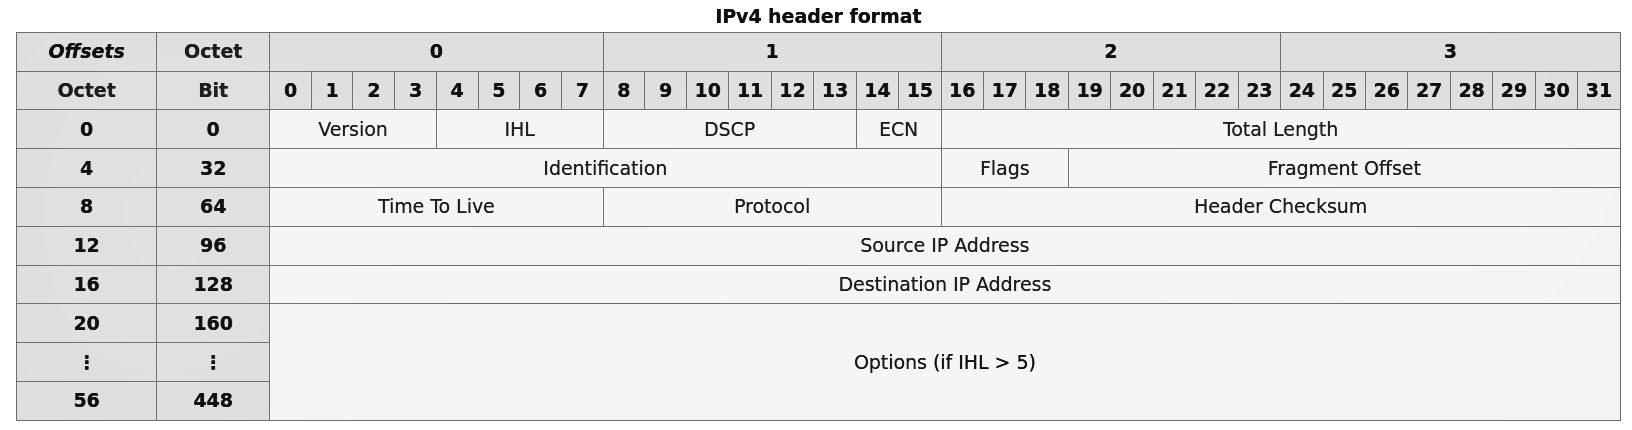
\includegraphics[ width=1.2\linewidth, height=\textheight, keepaspectratio]{./pics/tcp/ipHeader.png}
    \caption{Header of an IP packet. Source: Wikipedia.}
    \label{fig:ipHeader}
\end{figure}

Figure~\ref{fig:ipHeader} shows the structure of an IP packet. Essentially,
\begin{description}
    \item[Version, 4 bit] The first header field in an IP packet is the four-bit version field.
        For IPv4, this is always equal to $4$;
    \item[Internet Header Length (IHL), 4 bit] The IPv4 header is variable in size due to
        the optional 14th field (options). The IHL field contains the size of
        the IPv4 header, it has 4 bit that specify the number of 32-bit words
        in the header. The minimum value for this field is 5, which
        indicates a length of $5 \times 32 b = 160 b = 20 B$. As a 4-bit
        field, the maximum value is 15, this means that the maximum size of the
        IPv4 header is $15 \times 32 \mbox{ bit } = 480 \mbox{ bit } = 60 \mbox{ bytes }$.;
    \item[Differentiated Services Code Point (DSCP), 6 bit] Originally defined as the
        type of service (ToS), this field specifies differentiated services
        (DiffServ) per \texttt{RFC 2474}. Real-time data streaming makes use of the
        DSCP field. An example is Voice over IP (VoIP), which is used for
        interactive voice services;
    \item[Explicit Congestion Notification (ECN), 2 bit] This field is defined in \texttt{RFC
        3168} and allows end-to-end notification of network congestion without
        dropping packets. ECN is an optional feature available when both
        endpoints support it and effective when also supported by the
        underlying network;
    \item[Total Length, 16 bit] This 16-bit field defines the entire packet size in
        bytes, including header and data. The minimum size is 20 bytes (header
        without data) and the maximum is $65535 B$. All hosts are required
        to be able to reassemble datagrams of size up to $576 B$, but most
        modern hosts handle much larger packets. Links may impose further
        restrictions on the packet size, in which case datagrams must be
        fragmented. Fragmentation in IPv4 is performed in either the sending
        host or in routers. Reassembly is performed at the receiving host;
    \item[Identification, 16 bit] This field is an identification field and is
        primarily used for uniquely identifying the group of fragments of a
        single IP datagram. Some experimental work has suggested using the ID
        field for other purposes, such as for adding packet-tracing information
        to help trace datagrams with spoofed source addresses, but \texttt{RFC 6864}
        now prohibit any such use;
    \item[Flags, 3 bit] A three-bit field follows and is used to control or
        identify fragments. They are (in order, from most significant to least
        significant):
        \begin{itemize}
            \item bit 0: Reserved; must be zero;
            \item bit 1: Don't Fragment (DF);
            \item bit 2: More Fragments (MF).
        \end{itemize}
        If the DF flag is set, and fragmentation is required to route the packet,
        then the packet is dropped. This can be used when sending packets to a host
        that does not have resources to perform reassembly of fragments. It can
        also be used for path MTU discovery, either automatically by the host IP
        software, or manually using diagnostic tools such as ping or traceroute.
        For unfragmented packets, the MF flag is cleared. For fragmented packets,
        all fragments except the last have the MF flag set. The last fragment has a
        non-zero Fragment Offset field, differentiating it from an unfragmented
        packet;
    \item[Fragment offset, 13 bit] This field specifies the offset of a particular
        fragment relative to the beginning of the original unfragmented IP
        datagram in units of eight-byte blocks. The first fragment has an
        offset of zero. The $13$ bit field allows a maximum offset of $(213 –
        1)\times 8 = 65528 B$, which, with the header length included $(65528 +
        20 = 65548 B)$, supports fragmentation of packets exceeding the maximum
        IP length of $65535 B$;
    \item[Time to live (TTL), 8 bit] An eight-bit time to live field limits a
        datagram's lifetime to prevent network failure in the event of a
        routing loop. It is specified in seconds, but time intervals less than
        1 second are rounded up to 1. In practice, the field is used as a hop
        count—when the datagram arrives at a router, the router decrements the
        TTL field by one. When the TTL field hits zero, the router discards the
        packet and typically sends an ICMP time exceeded message to the
        sender. The program traceroute sends messages with adjusted TTL values
        and uses these ICMP time exceeded messages to identify the routers
        traversed by packets from the source to the destination;
    \item[Protocol, 8 bit] This field defines the protocol used in the data portion of
        the IP datagram. IANA maintains a list of IP protocol numbers as
        directed by \texttt{RFC 790};
    \item[Header checksum, 16 bit] The 16-bit IPv4 header checksum field is used
        for error-checking of the header. When a packet arrives at a router,
        the router calculates the checksum of the header and compares it to the
        checksum field. If the values do not match, the router discards the
        packet. Errors in the data field must be handled by the encapsulated
        protocol. Both UDP and TCP have separate checksums that apply to their
        data. When a packet arrives at a router, the router decreases the TTL
        field in the header. Consequently, the router must calculate a new
        header checksum;
    \item[Source address, 32 bit] This field is the IPv4 address of the sender of the
        packet. Note that this address may be changed in transit by a network
        address translation device;
    \item[Destination address, 32 bit] This field is the IPv4 address of the receiver
        of the packet. As with the source address, this may be changed in
        transit by a network address translation device;
    \item[Options, up to 288 bit] Options are largely unused, and may be considered harmful by
        some router. This is the portion of the IP header that is variable in
        size.
\end{description}


\begin{figure}[h]
    \centering
    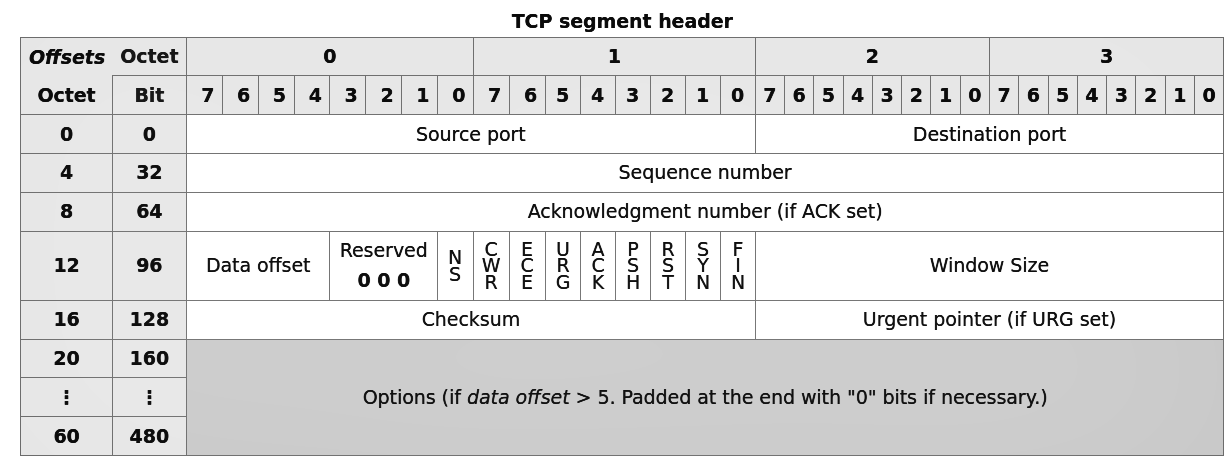
\includegraphics[ width=1.0\linewidth, height=\textheight, keepaspectratio]{./pics/tcp/tcpHeader.png}
    \caption{Header of a TCP segment.}
    \label{fig:tcpHeader}
\end{figure}

On the TCP header, instead, Figure~\ref{fig:tcpHeader} shows the header
structure,

\begin{description}
    \item[Source port, 16 bit] Identifies the sending port;
    \item[Destination port, 16 bit] Identifies the receiving port;
    \item[Sequence number, 32 bit] Will be covered later, its role is to keep
        track of the sequence of segments;
    \item[Acknowledgment number, 32 bit] Same as the above, but keeps track
        of the \emph{successfully delivered} packages;
    \item[Data offset, 4 bit] Specifies the size of the TCP header in 32-bit
        words. The minimum size header is 5 words and the maximum is 15 words
        thus giving the minimum size of 20 bytes and maximum of 60 bytes,
        allowing for up to 40 bytes of options in the header. This field gets
        its name from the fact that it is also the offset from the start of the
        TCP segment to the actual data;
    \item[Reserved, 3 bit] For future use and should be set to zero;
    \item[Flags, 9 bit] Contains $9$ flags, with some important ones:
        \begin{description}
            \item[URG] Indicates that the Urgent pointer field is significant;
            \item[ACK] Indicates that the Acknowledgement field is significant. All
                packets after the initial SYN packet sent by the client should have
                this flag set;
            \item[PSH] Push function. Asks to push the buffered data to the
                receiving application;
            \item[RST] Resets the connection;
            \item[SYN] \emph{Synchronize sequence numbers}. Only the first packet sent
                from each end should have this flag set. Some other flags and
                fields change meaning based on this flag, and some are only valid
                when it is set, and others when it is clear;
            \item[FIN] Last packet from sender.
        \end{description}
    \item[Window size, 16 bit] The size of the \emph{receiving window}. It is
        the number of window size units that the sender of this very segment is
        willing to receive. Useful in flow control;
    \item[Checksum, 16 bit] Checksum for error\--checking;
    \item[Urgent pointer, 16 bit] If the URG flag is set, then this 16-bit
        field is an offset from the sequence number indicating the last urgent
        data byte;
    \item[Options, variable 0–320 bit, in units of 32 bit] Various options.
\end{description}

\subsection{TCP Architecture}

\subsubsection{TCP bears an unpredictable and unrepeatable nature}

TCP carries many different implementations, depending mostly on OS of choice.
Several variants of its components have been written, with many of them largely
optional, or deprecated. As already mentioned, execution flow at application
level works independently and unpredictably with respect to the TCP-level flow:
when an application sends something, multiple TCP packages are exchanged;
how many and when they are sent is \emph{not predictable}.

TCP works by first copying data that should be sent in a buffer, and then send
them later.

The sequence of bytes is first copied to a buffer (sliding window) and the
\texttt{send()} function is, for example, invoked \--- the exact time in which a
segment is sent is \textbf{unpredictable}, \textbf{unrepeatable} and depends on
many things, over which the application has little to no control. This means
that application cannot \emph{deterministically predict} the exact time in
which the transmission will occur \--- instead, the TCP layer will deliver the
payload at a specific time determined by the protocol\footnote{However, also on
TCP layer there is a level of unpredictability. Many more effects can concur: for
instance, the Operating System may not be ready to send a segment, or may be
busy with other resources. These situation will cause delay in sending
information, even from the TCP layer's point of view.}.

On TCP, various \emph{events} can induce a transmission of data:

\begin{itemize}
    \item application invokes \texttt{send()} \--- in this case, the data in
        send's call argument will be inserted into the proper transmission
        buffer, and it will be transmitted somewhere in the (possibly
        immediate) future; 
    \item application invokes \texttt{receive()} \--- this way, we will see in
        detail that the TCP protocol will send a \emph{response} that
        \emph{acknowledges} the receipt of a segment, for the other party's
        sake;
    \item TCP layer \emph{receives a segment} \--- the same as above;
    \item a \emph{timeout} occurs \--- TCP layer will inform the other party of
        this;
\end{itemize}

Each of the above will trigger a transmission either immediately or
\emph{withing a maximum predefined time} (in the case of a timeout, for
instance). When a TCP layer ``is touched'' from above or below, \textbf{it reacts
by transmitting a segment}. Transmission should occur \emph{even if there is no
useful data to transmit} (e.g. if the transmission buffer is empty) \-- in that
case, a segment will only carry the header, which has information useful to the
protocol itself. Basically, regardless of the presence of data in the
transmission buffer the TCP protocol will exchange vital protocol information.
Protocol information is, in fact, necessary to keep the connection alive and
well-performing.

Upon transmission, TCP may deliver a varying number of bytes, ranging from
empty up to a number of bytes \emph{larger than Maximum Segment Size} ($536$ in
Internet network, $1460$ for same Ethernet network). Since huge payloads cannot
fit into a single segment with a predefined MSS, the TCP protocol
\emph{fragments} them before delivery, resulting in \emph{multiple segments
delivered in sequence}. TCP protocol will try its best to send as many segments
as possible, for efficiency's sake: it is not uncommon that $2$ or $3$ segments
are initially delivered before receiving the other party's response.

\begin{table}[ht]
\centering
\begin{tabular}{cc}
CPU Cycle & $0.3 ns$ \\
Main Memory Access (DRAM) & $120ns$ \\
SSD & 50-150 $\mu s$ \\
HHD & $10 ms$ \\
Internet, San Francisco to New York & $40ms$
\end{tabular}
\caption{Some interesting metrics. Notice the order of magnitudes differences
between CPU cycles and network delays. This table highlights the fact that
bytes cannot be injected through the internetwork at full\--speed: suppose one
has a $100MB$ transmission buffer that is delivered across just $1ms$ \--
injected throughput would be $100 \cdot 10^6 \cdot 8 b/(10^{-3} s)$, which
yields an astonishing $8 \cdot 10^{11} b/s = 800 Gb/s$, unsustainable for most
of internetworks.}
\label{tab:SomeMetrics}
\end{table}
\bigskip

The TCP protocol starts with \emph{slowly sending segments, increasing the exchange
speed as the time goes on}. Acceleration mainly depends on the timing of
\emph{received} segments, by looking at the metrics of confirmation packets
from receiver. As the sender acknowledges that the receiver is able to keep up
with the increasing transmission speed, it raises up the delivery speed. Basically, TCP layer adapts its speed to $2$ determining factors,
\begin{itemize}
    \item the receiver's speed at processing packages;
    \item the internetwork's capability of deliver packages.
\end{itemize}

As we will see in following chapters, the first factor is handled by the
\textbf{Flow Control} algorithm, while the second one is kept under control by
the \textbf{Congestion Control} system.

\subsubsection{How an application asks for data to be transmitted}

The system call \texttt{send()} processes the data transmission through the
network. The \texttt{send} function passes a memory buffer contained in
application space (address, length), and copies bytes from transmission memory
buffer in application space to transmission memory buffer in TCP layer (called
\textbf{TX-buffer}).

\begin{lstlisting}
public void write(byte[] b)
	throws IOException
\end{lstlisting}

Send is first invoked by application level, whose execution flow is completely
independent from the TCP layer's one. Buffer at application layer is then
copied to the TCP transmission buffer, to be sent immediately or later. New
invokations of \texttt{send()} will copy data in TCP buffer \textbf{after} the
data that is already present.

Invoking \texttt{send()} \textbf{does not guarantee} any immediate
transmission: all it does is pushing application data into TX-buffer to be sent
in future. TCP will then \emph{independently} establish the proper moment and
way to transmit data present in transmission buffer.

Suppose now one has to send $N$ bytes with $K$ consecutive \texttt{send()}
invocations. How many segments will be exchanged? How many transmission events?

First and foremost, the number of segments will not depend on $K$, since no
matter how many times \texttt{send()} is invoked, the end result will be to simply
insert those $N$ bytes in the TX-buffer, because the sole effect of
\texttt{send()} is to insert the passed number of bytes into the TX-buffer,
triggering a transmission. As a first approximation, the number of transmitted
segments will roughly be $$\mbox{\#transmitted } = \frac{N}{MSS} + 1,$$ with
the last segment $+1$ smaller than the previous ones. Things, however, can go
wrong and be much more complex due to packet loss and retransmissions. Recall
that for all these reasons, the exact number is neither predictable nor
repeatable.

\subsubsection{Retrieving data from TCP}

Data retrieval occurs with another system call, \texttt{receive()}. System call
\texttt{receive()} is quite similar to the \texttt{send()} call: both
receiver's TCP layer and Application layer execution flows act independently to
each other, and receiving buffer is not guaranteed to contain any data.

When data reaches the receiver, the data is copied into the receiving buffer
(\textbf{RX-buffer}). The receiving buffer stores all received bytes and is
flushed only when the application invokes \texttt{receive()}. The function
\texttt{receive()} copies (at least a portion of) the receiver buffer into the
application buffer by means of passing a buffer with known \emph{address} and
\emph{length}. Function \texttt{receive()} copies bytes without exceeding the
size of the buffer (\emph{length}) and it \textbf{returns} how many bytes have
been copied into the provided buffer. As argument, \texttt{receive()} also
takes the number of bytes to fetch from the TCP receiving buffer. Basically,
\texttt{receive()} needs to accept a buffer to which data should be copied, its
length (in C length information is \textbf{not} intrinsic to arrays) and the
expected number of bytes to be retrieved.

There are three possible outcomes for the \texttt{receive()} call:

\begin{itemize}
    \item the \emph{receive buffer is empty}: the application is suspended and
        the process is put to sleep until some data is available;
    \item \emph{more than \texttt{length} bytes are available}: a
        \texttt{length} number of bytes is fetched and delivered to the
        application as soon as possible. More \texttt{receive()} calls are
        needed to retrieve all data and empty the RX-buffer;
    \item \emph{less than \texttt{length} bytes are available}: all available
        bytes are copied as soon as possible, since they are less than the
        maximum deliverable value. The single \texttt{receive()} call will not
        yield all requested bytes, and more calls should be used.
\end{itemize}

Basically, each time a number of bytes is requested, TCP will provide \emph{up
to} that number of bytes. The application is held back only in the case when there
is no data available.

Now with an example: let a buffer have length equal to $800$ bytes. Suppose
\texttt{receive()} is invoked in the following scenarios,
\begin{enumerate}
    \item in the first scenario, there are $600$ bytes in the RX-buffer. Upon
        \texttt{re\-cei\-ve()} call, all $600$ bytes are delivered to the
        application. The RX-buffer is now empty;
    \item in the second scenario, there are $1000$ bytes in the RX-buffer. Upon
        \texttt{receive()} invocation, only $800$ of the $1000$ bytes are saved
        into the buffer \-- $200$ bytes will remain into the RX-buffer;
    \item in the third scenario, there is \emph{no data} in the TX-buffer.
        Application is suspended until there is data to retrieve. Suppose $500$
        bytes are collected in the RX-buffer \-- they will be immediately saved
        into the buffer provided by the application, and the application will
        retrieve them. RX-buffer is now emptied.
\end{enumerate}


\subsection{Sequence numbers}

IP protocol is \emph{unreliable} (packets can be lost, duplicated, or delivered
in different order from which they were sent). To overcome this huge
shortcoming, each data byte is implicitly identified by a $32$ bit
\textbf{sequence number}\marginpar{\small\textsf{Sequence number}}. A sequence number is a label for each transmitted and
received byte, so that both correct ordering and amount of data can be properly
determined. The association is \emph{implicit} \--- the sender applies a
sequence number to a segment, and the receiver uses that information to
reconstruct the original order of segments. This way, segments are
reconstructed even if they show up haphazardly, and the data can be assembled
as it originally was.

There are many variables\marginpar{\small\textsf{snd.User}} involved in sequence numbers. \texttt{snd.User} is the
variable carrying the value of the next byte the \textbf{application} will
send. The variable \texttt{snd.Next}\marginpar{\small\textsf{snd.Next}} carries the value of the next byte that
the \textbf{TCP layer} will transmit \--- its value is contained in the TCP
header (initial byte of the sequence, of course). Basically, \texttt{snd.User}
refers to the next byte that will be filled by the invocation of
\texttt{send()}, while \texttt{snd.Next} is the next byte yet to transmit by
the TCP layer. The sequence number of application level must be computed from
other information. 

The variable \texttt{snd.Next} is carried in the TCP segment header, in
\emph{sequence number} space (16 bit).

In short,

\begin{itemize}
	\item \texttt{snd.Next} is the boundary between transmitted data and
		yet-to-transmit data;
	\item \texttt{snd.User} is the boundary between in TX-buffer data (data
        sent by application) and not-yet-associated bytes, the free space in
        the buffer.
\end{itemize}

Upon sending a segment, the \emph{sequence number} will be inferred from the
\texttt{snd.Next} variable, and will be the \emph{next byte the other endpoint
expects}.

\begin{figure}[b]
        \centering
        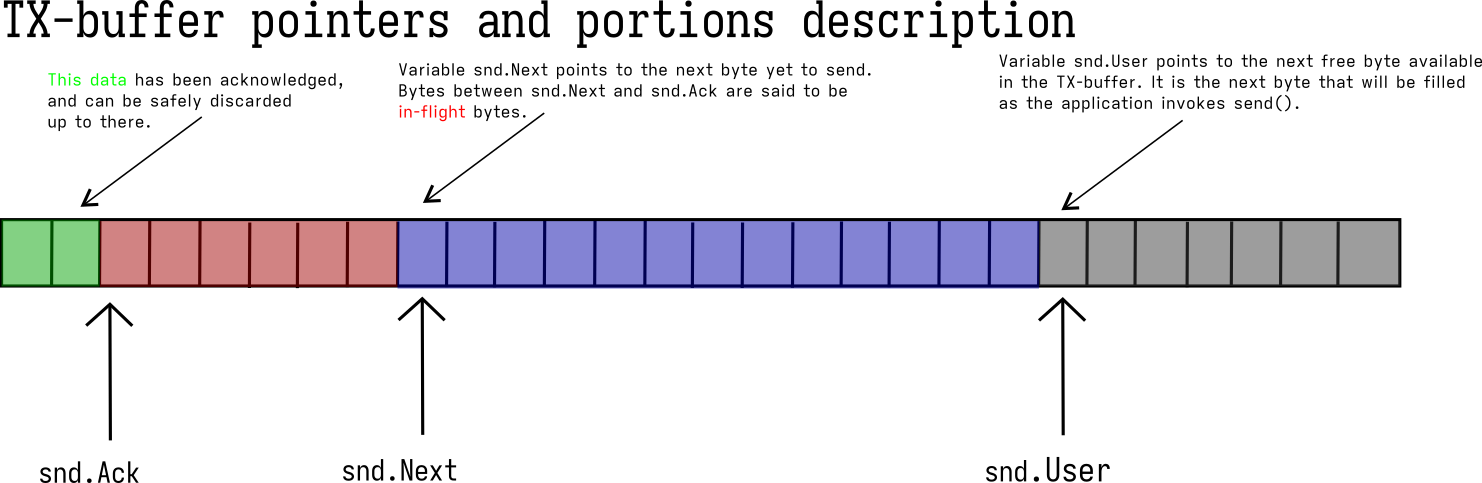
\includegraphics[ width=1.2\linewidth, height=\textheight, keepaspectratio]{./pics/tcp/TxBuffer.png}
	\caption{TX-Buffer and its flags \texttt{snd.Ack}, \texttt{snd.Next} and \texttt{snd.User}.}
        \label{fig:TxBuffer}
\end{figure}

From the receiver's point of view, the variable \texttt{rcv.Next} is the
boundary between content of RX-buffer and not-yet-received data (right boundary
of the data currently in buffer). The variable \texttt{rcv.Next} is similar to
the variable \texttt{rcv.Next} in the sense that it points at the next byte yet
to receive. Only packets having the \emph{expected sequence number} are collected
and brought into the buffer.

There is a special case where some segment carries new parts of information and
sequence numbers that are not collected, with a portion of them already
collected: in that case the incoming segment will still be collected, with
duplicated bytes thrown away. There may be two reasons for packet duplications:
either IP layer duplicates them, or the TCP sender retransmits them because it
thought they were lost. In order to be able to retransmit packets, TCP stores
all sent data in buffer until acknowledgement has been received, since they
could be retransmitted in the immediate future.

\begin{itemize}
    \item \texttt{rcv.Next} points at the next byte that is not yet being
        received;
    \item \texttt{rcv.User} points to the next byte to be received by the
        application. After \texttt{receive()} invokation by the application,
        all bytes that have been successfully delivered to the application can
        now be safely deleted.
\end{itemize}

\begin{figure}[b]
        \centering
        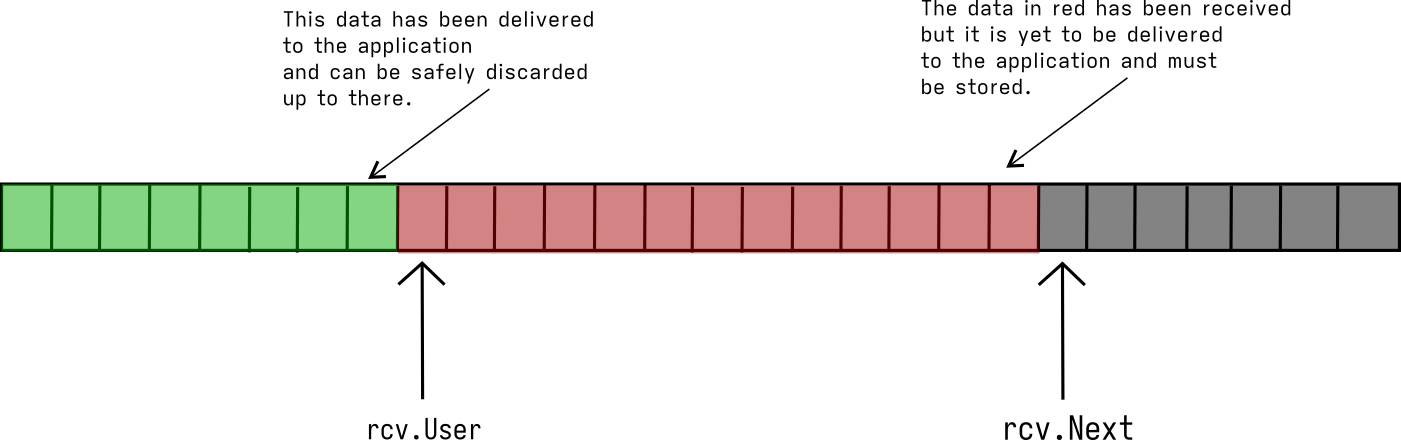
\includegraphics[ width=1.0\linewidth, height=\textheight, keepaspectratio]{./pics/tcp/RxBuffer.png}
    \caption{RX-buffer and its flags. Notice that RX-buffer only uses two flags
    instead of three (no ACK flag needed). Indeed, there is no need to keep
track of sent ACKs: they will be sent as soon as segments are acquired.}
        \label{fig:RxBuffer}
\end{figure}


Each TCP layer has \textbf{both} TX-buffer and RX-buffer. Sequence numbers in
the two directions are independent each other, and they will increase as much
as there is new data incoming from a direction.

Each and every segment is accepted only if it contains \emph{new} data: that
is, when the sequence number is the expected one \emph{or} when the segment
contains novel sequence numbers. 

Each segment also carries information on the \emph{length} of its payload. This
allows the receiver to efficiently reconstruct the segment, in order to compute
the ending sequence number, and not only the starting sequence number.

An important remark is that \textbf{sequence numbers are 32-bit integers}.
Therefore, the sequence numbers can only go from $0$ to $2^{32} - 1$, so there
may be \emph{wrap-arounds} in an overflow-like fashion. TCP should internally
handle these comparisons in a proper manner.

\subsection{Handling duplicates and loss}

IP is an unreliable protocol. This means that \emph{packets can be loss}.
Necessary mechanisms are two,

\begin{itemize}
    \item the \textbf{retransmission}, or when a segment is regarded to be
        sent again;
    \item the \textbf{acknowledgement}, which is a kind of \emph{notification
            of receipt}, that is sent by the receiver in order to make the
            other party sure that it has received and collected the data sent
            to it.
\end{itemize}

\emph{Acknowledgements} are a mechanism that assures receipt of a message by
means of \emph{notifications}. Every header of a segment contains the sequence
number of \texttt{snd.Next}. Every segment also \emph{carries an information
regarding the bytes that are received}: the \textbf{acknowledgement number},
which tracks the state of the RX-buffer by following the pointer
\texttt{rcv.Next}. This way, having both sequence number and acknowledgement
number, one can successfully track the state of a TCP connection. Upon sending
a TCP segment, both sequence number and acknowledgement number are delivered,
so that the receiver can reconstruct the state of the sender RX-buffer.

Basically, sequence number tracks the bytes a party \emph{has sent}, while
acknowledgement number tracks the bytes a party \emph{has successfully
received}. Both informations must be exchanged at every delivered segment.

A fifth variable\marginpar{\small\textsf{snd.Ack}} is thus needed: \texttt{snd.Ack}, which \emph{points to the
byte in TX-buffer before which any transmitted byte had been acknowledged}.
This variable is only increased upon receiving data (for instance, upon
receiving a sequence with a greater ACK number from the sender). Since it has
been safely collected, all data before \texttt{snd.Ack} pointer can be
forgotten. 

Acknowledgements mechanism is crucial to a TCP connection, in order to
provide \textbf{reliability} to a connection. Therefore, transmission of
acknowledgements is always necessary even if TX-buffer is empty. In that case, no
payload will be transmitted, and only protocol information is sent (increasing
acknowledgement number).

An important note is that \texttt{snd.Ack} is only updated when the received
sequence number \texttt{segment.ack} is \emph{greater} than the value in
\texttt{snd.Ack} \-- that is, when new data are correctly received.

For this reason one can say that the sequence number tracks \texttt{snd.Next},
while the acknowledgement number tracks \texttt{rcv.Next}. However, the
sequence number will be at the value of the \emph{first} sent byte, that is the
first byte the receiver is expecting.

For instance, suppose the receiver has successfully received $130$ bytes from a
sender: its \texttt{rcv.Next} points to the $130$th element in the RX-buffer.
In order to inform the sender, all the new incoming segments from the receiver
will carry $130$ as sequence number (it points to the $131$st element). Upon
receiving such packets, the sender will successfully interpret the sequence
number, and set the \texttt{snd.Ack} variable to $130$: all the data prior to
$130$ can be safely discarded.

Data bytes between pointers \texttt{snd.Ack} and \texttt{snd.Next} is said to
be \textbf{in flight} data. These bytes have been transmitted but not yet
acknowledged, and are potentially eligible for retransmission.

The reason why acknowledgements are important is pretty straightforward: without
acknowledgements, there would be \textbf{no way for the sender to tell whether
sent data has been received or not}. This means that even though the receiver
has no data, acknowledgements are still required and should be properly sent.

In the end, acknowledgements are a crucial component of TCP, without them it
wouldn't be possible to provide either a reliable or a predictable connection,
with no chance of keeping track of actually and successfully delivered
information.


\subsection{Delayed Acknowledgement}

\emph{Delayed Acknowledgement} is a notorious TCP algorithm. Its core idea is
not to answer immediately with an acknowledgement, but to await some arbitrary
time interval $T$ that depends on the operating system. The algorithm is pretty
straightforward:

\begin{quote}
Upon receiving a segment, if delayed-ack timer $T$ has previously been set,
\emph{transmit immediately}. Else, set the delayed-ack timer $T$ to a specific
value.
\end{quote}

When receiving a packet, simply set a timer, and send the response segment
after timer expires. However, if you receive yet another segment before the
timer expires, then send immediately the response.

Delayed-ack timer value depends on the operating system:

\begin{itemize}
    \item RFC suggests $T = 500ms$;
    \item Windows has $T = 200ms$;
    \item Linux in general has $T = 40ms$;
    \item RHEL sets $T = 4ms$.
\end{itemize}

The reasoning is as follows: if there is not much data to transmit, it will be
likely that the timer $T$ will expire. Expiring timer means sending a packet
with the proper acknowledgement number \-- a strategy that guarantees that the
connection stays open and remains fresh. If the other part is sending a lot of
data, the contrary will be more likely to occur, breaking the awaiting. In
order to help the other part, acknowledges will be delivered as soon as a
\emph{second segment} is received. 

The core idea is to both help the other end and
minimize the number of segments to be sent: this is done by preventing to
respond with a segment whose sole purpose is to inform of acknowledged data
\emph{at each segment received}, while still answering with ACK information
even though there is little to no data received. In fact, a delay time $T$
assured to save sending some segments, a feature that historically was of a
crucial importance.

\subsection{Retransmissions}

The connection state includes three more actors, related to
\emph{retransmission}:

\begin{itemize}
    \item a \textbf{retransmission timer}, which counts the time interval until
        which the retransmission is held back;
	\item a variable that describes the \emph{duration of retransmission
        timer interval}, the \textbf{RTO (Retransmission Time-Out)};
    \item a \textbf{retransmission counter}, that counts how many
        retransmissions for a segment have been performed.
\end{itemize}

The \textbf{retransmission algorithm} is as follows:

\begin{quote}
    Upon transmitting segment S, \emph{if timer is not already set}, then the
    counter is cleared and set to $0$, with the timer set to the RTO value.
    At the beginning, then, a new counter is spawned and the timer is set to
    a value which is the RTO value.

    When an ACK is received, \texttt{snd.Ack} is updated to the maximum value
    between \texttt{snd.Ack} and \texttt{segment.Ack}. If \texttt{snd.Ack ==
    snd.Next}, the timer is switched off: the sent data has been received by
    the other party correctly and as expected.

    There may be occasions in which the timer expires, though.
    When timer expires, the \emph{counter is incremented} and if the counter
    has not yet reached a \texttt{MAX\_COUNT} value, the segment is
    retransmitted. However, this time the timer value is set to RTO but
    \texttt{RTO = 2 * RTO}, which is the double of the original value.
    \emph{Only in-flight data should be retransmitted} (and all of it after
    timer expires). Basically, data for which we are sure that it has been
    received should not be retransmitted in case the timer expires, and the
    sender should only focus on retransmitting not-yet-acknowledged data. At
    each retransmission, the RTO is doubled, and the retransmission counter is
    increased.

    When counter reached \texttt{MAX\_COUNT} value, an excessive number of
    retransmissions has been attempted, and connection is closed.

    Upon receiving an ACK for \textbf{all} the in-flight data, switch the timer
    off (that is, when \texttt{snd.Ack == snd.Next}).

    A particular condition is when an ACK arrives \emph{for only a portion} of
    the data that has been sent. In that case, the timer resets (the receiver
    has responded) to the RTO value, \emph{as if those still not-ACKed had been
    sent now}, and the sender awaits ACK for missing segments. This basically
    occurs when a partial ACK comes, and prevents unnecessary retransmissions.
\end{quote}

Exact\marginpar{\small\textsf{Choosing RTO}} timings of retransmissions are hard to predict. A sender is completely
blind if it does not receive any ACK: should it send again in-flight segments,
or should it wait a little bit more? In practice, how long should the timer be
set? Basically, a rule of thumb is that it should be ``slightly larger'' than
Round\----Trip Time. In order to do so, since RTT largely varies depending on
connections, time, and many other conditions, RTO is \textbf{dinamically updated}
by algorithms such as \emph{Jacobson algorithm}.

Regarding the maximum number of retransmissions\marginpar{\small\textsf{Max\_Count}}, value of \texttt{MAX\_COUNT}
largely depends on the operating system. For instance, Windows closes
connection after $5$ failed attempts, Linux after $15$. It is simple to realise
that there may be a lot of unnecessary retransmissions: the timer can, for
instance, run out too soon for the acknowledgement to reach the sender.
Unnecessary retransmissions are a waste of resources, and definitely a
fundamental problem. The reason could be one of those:

\begin{itemize}
    \item segments are \emph{lost}, retransmissions are necessary;
    \item there could be segments \emph{whose ACKs are lost};
    \item RTO was set to a \emph{too small value}.
\end{itemize}

Thus, RTO should be set to an appropriate value, since a too short value leads
to high overhead and possibly many unnecessary retransmissions, while a too
long value results in high latency and possibly a slow or non-responsive
connection. RTO value is basically a \emph{trade-off} between exhibiting few
retransmissions and having a fast and responsive connection. RTO should be set
\textbf{dinamically}: it should be slightly greater than the \emph{RTT}
(Round-Trip-Time), an idea from Jacobson algorithm. This is of a crucial
importance for TCP to work. Initial RTO value is heuristical, and varies from
one OS to another. Linux and Window start from same value, macOS use a
different value, and so on.


\subsection{Multiple default gateways}

More default gateways could be added to a single node. Reasons to add more than
one default gateway all boil down to \emph{failure avoidance}. To know whether a
gateway has stopped working, a heuristic TCP algorithm tries to detect a
gateway failure:

\begin{quote}
    If the number of retransmissions is greater than \texttt{MAX\_COUNT}
    divided by 2, the \emph{connection} changes its default gateway (if
    possible). Moreover, if the number of connections that changed default
    gateway is greater than the number of open connections divided by 4, the
    \emph{IP layer} changes the default gateway as well. This last feature
    speeds up reconfiguration of early connections that still have to make some
    retransmission attemps.
\end{quote}

Basically, each connection can autonomously choose its own gateway, but the IP
layer is able to \textbf{force} any \--- new or already present \--- connection
to use a different default gateway. A connection that exceeds the total number
of retransmissions will change default gateway, and if $4$ or more connections'
default gateway switches are detected the IP layer will switch to a different
default gateway as well, forcing all newly created TCP connections to switch to
the new gateway.


\begin{figure}[h]
    \centering
    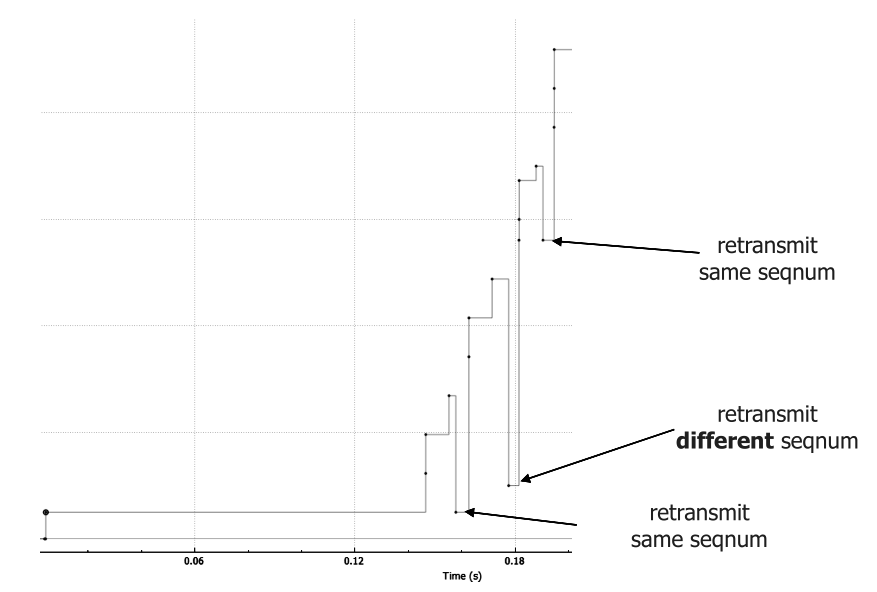
\includegraphics[ width=1.0\linewidth, height=\textheight, keepaspectratio]{./pics/tcp/timeSequenceTCP.png}
    \caption{Time plot of sequence numbers. Dots correspond to sent segments. Some retransmissions occur.}
    \label{fig:timeSequence}
\end{figure}

\subsection{Selective Acknowledgements}

Suppose that 4 segments are sent, and the second one has been lost: in this
case, the receiver got all segments except the second one, but it has
no way to inform the sender to retransmit only the second segment. Sending
ACK for only the first segment would result in unnecessary retransmission of
segments 3 and 4, which were instead correctly received. 

For this reason, the receive buffer could end up having some \textbf{gaps},
missing bytes that are supposed to be received. The solutions are
\textbf{Selective Acknowledgements} (SACK), a special kind of acknowledgements
that carry both \emph{left and right sequence number edges} of each
out-of-order \textbf{block} in RX-buffer, this way correctly informing the
other party of a \emph{specific} missing portion of the data, avoiding
unnecessary retransmissions. Selective Acknowledgements can selectively mark
which bytes should be transferred again, and only those.

SACK protocol must be \emph{supported by both members} of a connection in order
to be useful. The protocol is very convenient, since many segments can be lost
when a sender tries to deliver dozens of segments at once. This way, TCP can
achieve \emph{efficient handling} of the connection, minimizing the number of
unnecessary retransmissions.

In SACK\--supporting segments, a \texttt{TCP Option} field exist, in which both
\texttt{left edge} and \texttt{right edge} are inserted, and they allow for
correct data reconstruction after it has been lost, only for that portion
delimited by the two edges.

Of course, out-of-order segments could still lead to gaps in RX-buffer, causing
an unnecessary retransmission. In this case, unnecessary retransmissions are
unavoidable when an out-of-order segment reaches the receiver too late, after a
long time interval, since the receiver will send a SACK informing the sender of
the missing segment, while the very same segment arrives late. However, no
matter what, SACK is always convenient, since it reduces a lot the burden to
the sender for only missing segments are to be sent.

To optimize out-of-order gaps, \textbf{Fast retransmit} algorithm should be
adopted (not part of this course).

\subsection{Operating System TCP interrupts and the real TCP execution flow}

Upon packet arrival, a \emph{system interrupt} is sent. 

An operating system executes many concurrenct activities: application process, other networking processes, manages other system interrupts, and so on.

When a system interrupt is cast, the operating system will try its best to fetch data from the network physical device.

From the TCP point of view, after data comes from the operating system, he will
analyze the packet to sort it by \emph{looking at the connection table}, and
then it will \textbf{push in the input queue} the relative packet. The input
queue holds a certain amount of segments, stored in the order given by sequence
number.

When the TCP protocol decides it's time to process all segments in queue, it
deeply analyzses them, picks their payload, grabs their header information, and
processes all of them. After processing all segments in input queue, the buffer
is emptied.

Basically, TCP can never \textbf{immediately} process a segment upon arrival.
What it can do best, is to await some time, receive an amount of segments
depending on the operating system's load at that moment and many other factors,
and then process them altogether. Since many of them are processed at the same
time, only a single acknowledgement will be sent back to the sender.

Since there are \emph{many} different sources of randomness, let alone things
that are completely out of TCP's control (just think of connection's quality,
operating system's load, the other's end capabilities, packet loss,
send\----receive invocations), there is \textbf{no} single correct way for TCP
protocol to exchange a given amount of data with another party.

\section{Flow and Congestion Control}

To behave optimally, TCP needs to establish the correct amount of data that
should be exchanged in an interval of time.

Whenever TCP decides to transmit, there are three possible scenarios: 
\begin{enumerate}
    \item an empty segment is sent when there is no payload \-- that is the
        case, for instance, of acknowledgements or when timer expires;
    \item it transmits a single segment if payload data is smaller than MSS \--
        that is for few data;
    \item it transmits multiple segments if payload size exceeds MSS \-- that's
        the case for huge payloads.
\end{enumerate}

However, not all connections are equally good, and not all endpoints are fast
enough to cope with a sender's speed. A sender should not send more segments
than how many can be managed by the receiver \--- \emph{how many} is an upper
limit that should be dynamically changed.

The overall idea is the following one: TCP \textbf{starts slowly}, then
\emph{increases its transfer speed} according to the rate in which
acknowledgements are received. Since the interaction is bidirectional and
quite complicated, TCP implementation at sender's side tries to adapt to
both connection properties and receiver's side properties. 

As a general rule, the number of in-flight bytes is \emph{always lower than an
upper bound that is dynamically updated}, with an upper bound that is chosen
according to proper criteria. This means that TCP can automatically
\emph{adapt} to the peculiar characteristics of the connection and receiver's
speed.

In order to adapt the two different aspects of a TCP connection \-- the
\emph{connection quality} and the \emph{receiver's speed} \-- two bounds should
be adopted: the \textbf{Flow Control} and the \textbf{Congestion Control}. The
TCP layer will always send less data than the minimum between the two upper
bounds. 

The first algorithm constructs a bound in such a way that the capacity of the
receiver is always respected. Let an extremely fast computer send data faster
than a receiving, slow, computer. Slower computer has not enough speed to
collect all data that has been sent \--- the flow control algorithm lets the
sender speed adapt to the receiver speed by means of a \emph{send window}. 

The second algorithm, the congestion control, constructs a state variable
called \emph{congestion window}, whose goal is to \emph{model the maximum current
throughput of the network}. 

The number of in-flight bytes \emph{must be slower than both send window and
congestion window multiplied by MSS}, so that $$\mbox{in-flight} \leq
\min(\mbox{sndWin}, \mbox{congWin} \cdot \mbox{MSS}).$$ 

The mental model should be the following one: if the transmission buffer is
full of data, a number of in-flight bytes equal to the minumum of both
quantities should be sent, otherwise just send \texttt{snd.User - snd.Ack}
bytes (those still to send).

\subsection{Flow control}

Buffers cannot increase indefinitely: boundaries must be set in order to assure
system stability. In Linux kernel, buffer sizes are set upon compilation and are
then fixed; different operating systems may show other behaviors. In case data
cannot be pushed into the TX-buffer anymore because it is full, application
should be suspended. When the RX-buffer is full, packets have to be discarded
since they cannot be collected. Flow control will act to prevent this situation
by letting the sender know how much free space is available to the RX-buffer. 

The goal of flow control is to keep a fast transmitter from overrunning a
slower receiver.

Since application sends data much faster than ACK arrive, the TX-buffer could
end up being filled up by incoming segments. Suppose at receiver's side the
application invokes \texttt{receive()} much slower than incoming packages
speed. This way, the RX-buffer could fill up as well. To solve this issues,
application invokes \texttt{send()} only when TX-buffer is full, hence it is
put to sleep (blocked) until TCP gets proper ACK and advances \texttt{snd.Ack}
(when it has more free space).

TCP sender keeps track\marginpar{\small\textsf{Window Size}} of free space in other end's RX-buffer by looking at a
variable in header (WindowSize) that informs it of how much free space is
available, so that it can actually predict how much free space there is. When
it guesses that receiver's RX-buffer could have no space left, it stops
transmission and suspends the application. If the maximum window corresponds to
the size of a single segment, the protocol is called \textbf{stop-and-wait}
(that is \-- send a single segment, than wait for ACK). Larger windows enable
pipelining of multiple segments in a row, allowing far more efficient usage of
the connection.

Flow control algorithm\marginpar{\small\textsf{Sliding Window}} adopts the concept of \textbf{sliding window}. Each
segment header has a \texttt{WindowSize} field in the header that contains
\emph{how many free bytes are in the RX-buffer}. From sender's point of view,
\texttt{snd.winSize} contains the \emph{number of free bytes in RX-buffer of
the other side}.

The value is initially set to the receiver's entire buffer size, and it is
updated dynamically upon sending a segment. If a segment \texttt{S} carries
\texttt{S.Ack} that is greater or equal to \texttt{snd.Ack}, then the variable
\texttt{snd.winSize} is updated and set to \emph{S.windowSize}. The
\texttt{snd.WinSize} value ranges from $0$ to the buffer size at the receiver's
end.

Ultimately, the number of in-flight bytes must never exceed the number of bytes
in \texttt{snd.winSize} that are available in the RX-buffer. This means that
\texttt{snd.Next - snd.Ack} should \textbf{never} be greater than
\texttt{snd.\-WinSize}.

The end goal of TCP is to reach a number of in-flight bytes that is as close as
possible to the \texttt{snd.winSize} number of bytes, in order to optimize the
connection efficiently.

\begin{figure}[b]
    \centering
    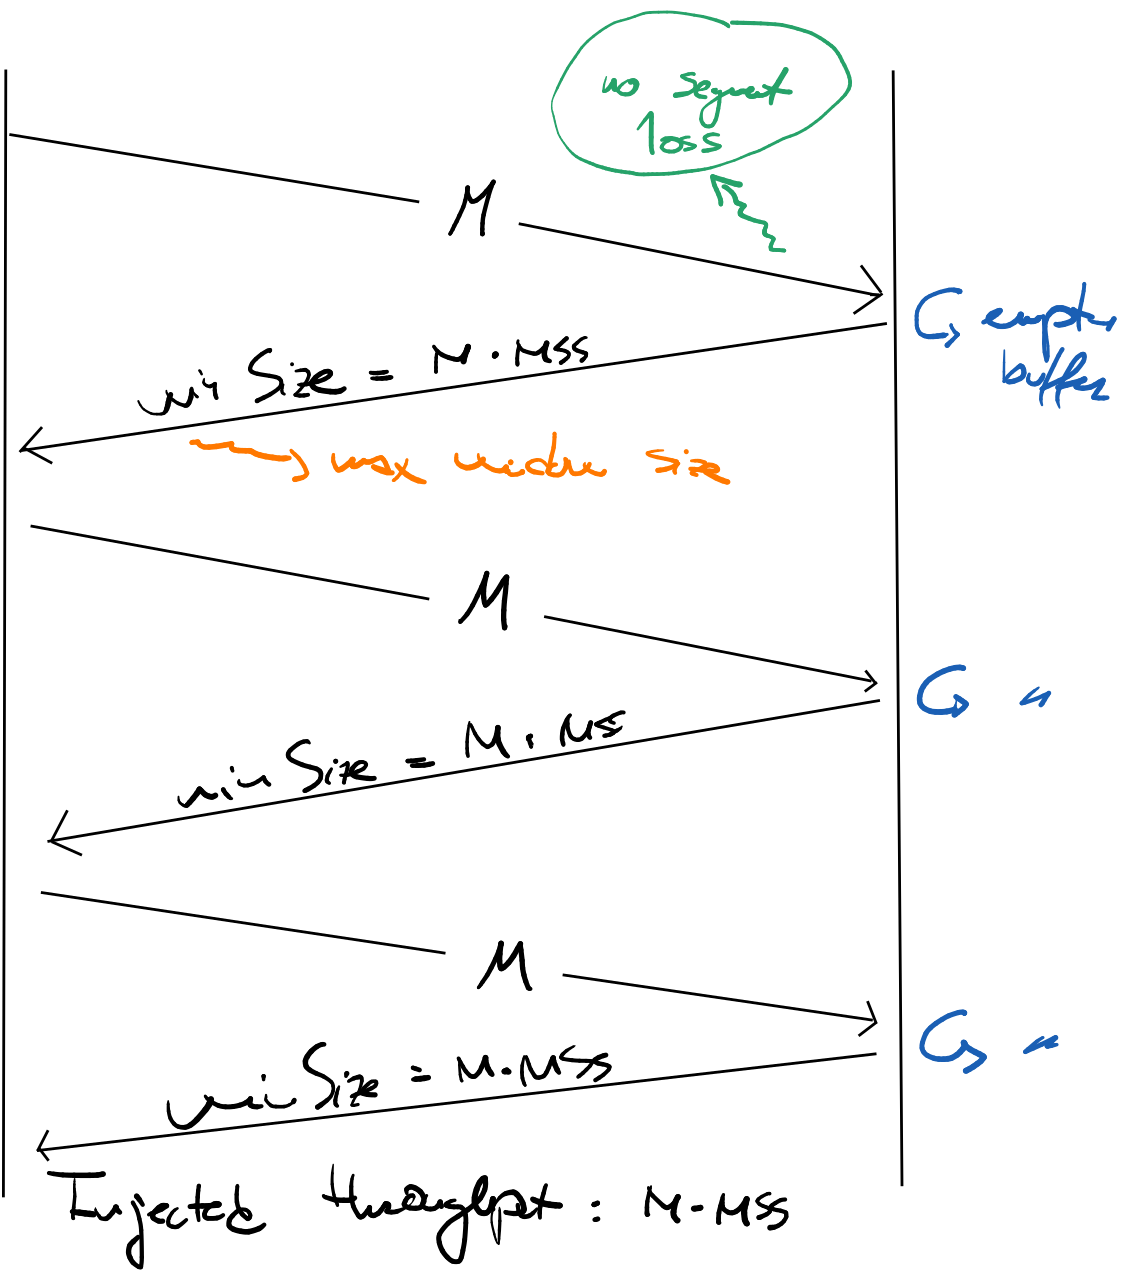
\includegraphics[ width=1.0\linewidth, height=\textheight, keepaspectratio]{./pics/tcp/idealThroughput.png}
    \caption{Ideal throughput condition, in which the injected throughput is
    equal to M $\cdot$ MSS at each time $T$. In scheme, every timing is
considered constant, and the total time $T$ is the sum of the time in which all
the segments arrive at the receiver's end, the receiver's processing time and
the acknowledgement's time to arrive at the original sender's side.}
    \label{fig:idealThroughput}
\end{figure}

\clearpage


\subsection{Performance estimation}

From flow control, let's determine the maximum T-IN-TCP (input throughput) that can be obtained.
TCP is injecting some throughput into the network, and the amount of it is
controlled by the flow control algorithm. 

Suppose the receiver has a window size of $M \cdot MSS$, and the application
requesting data invokes \texttt{receive()} on a large buffer, such that the
buffer is emptied as soon as there is new data.

The best case one can get by flow control is $M \cdot MSS$ every RTT \--- this is
the case where the receiver's application empties the RX-buffer the moment the
segments arrive. Suppose in fact $M \cdot MSS$ bytes are sent at each round,
and no packet loss occurs: in that case, the receiver would immediately and
successfully grab all segments, sending the corresponding acknowledgment
answer.

In the case the application empties \emph{half} the buffer at periodic
intervals, the throughput would be the half as well, $M/2 * MSS$ every RTT.
After the first round, only half of the segments would be sent, since the
window size is indeed the half of the total one. 

If the entire buffer is emptied at once, but with a delay, or not aligned with
the receipt of segments, the throughput would be $M * MSS$ every RTT + $\Delta$
(more time than plain RTT). Combining all cases, one could get less than $M *
MSS$ data every \emph{longer} than RTT, depending on the parameters and the
circumstances of the network.

For the best case, it's important to recall that some important assumptions
have been made:
\begin{itemize}
    \item all intervals have same time duration $T$, as described in
        Figure~\ref{fig:idealThroughput};
    \item all the segments arrive together, or at least not after a time which
        is irrelevant or already counted in $T$.;
    \item acknowledgement arrives immediately, and not after a huge delay;
    \item receiver is perfect in managing segments, and provides an
        acknowledgment segment for the full data.
\end{itemize}

In every case, a greater RX-buffer will result in higher throughput, since
there is a proportionality between throughput and buffer size. Viceversa,
greater RTT will result in less throughput \--- LANs will have greater
throughput than WANs since they possess a lesser Round\----Trip Time. However,
in this formula the \emph{quality} of the network is not taken in account:
segments can be loss, especially when too many of them are injected through the
internet. For this reason, this much-optimistic model cannot be applied in
cases where the throughput is high (read \--- when RX-buffer is insanely huge).
Every time a retransmission is needed, \emph{detection and recovery} takes
place, and throughput becomes much smaller than the ideal case. This
phenomenon is much heavier as the RTT increases, since retransmissions are
harder to assess; Moreover, it is far from being predictable.

Another thing to consider is \emph{maximum network speed}. Injected throughput could
be \emph{even greater} than maximum network speed, in that case many segments
would be loss, resulting in a sub-optimal efficiency\footnote{This is solved by
Congestion control mechanism.}.

\subsubsection{Establishing size of RX-buffer}

Size of RX-buffer\marginpar{\small\textsf{Receiver's Buffer Size}} should have the following characteristic: the size should be
\emph{a multiple of MSS} \--- this is done to avoid leaving unused space at the
end of the buffer, since in the lucky case exactly a multiple of MSS will be
delivered. Non\--multiple sizes would make no sense.

However, the RX-buffer size is a \emph{trade-off} between greater ideal
throughput and lower throughput due to excessive retransmissions, and should be
chosen accordingly. Unexpectedly, $64KB$ are chosen; the value is OS-dependent.
The size is managed as if it were a multiple of MSS \--- when almost full,
pretend it is full and ignore last portion of buffer.

\begin{table}[ht]
\centering
\begin{tabular}{ccc}
    Flow control & Ethernet & Internet \\
    MSS  & $1460B$ & $536B$ \\
    RX-buffer & $64KB$ & $64KB$ \\
    number of segments in-flight & $44$ & $122$
\end{tabular}
\caption{Quantities involved in flow control, on Ethernet and Internet.}\label{tab:FlowControlQuantities}
\end{table}
\bigskip

\subsection{Sustainable throughput}

A sustainable throughput is indeed \textbf{not infinite}. After a certain injected
throughput \texttt{T\_MAX}, the network bottlenecks and starts losing segments, exhibiting a
behavior that will lead to less performance. Thus, an optimal throughput should
be determined by and largely depends on \emph{connection quality}. Injected
segments are delivered at same speed only if the injected throughput is lower
than the maximum possible throughput, that is \texttt{T\_MAX}.

\begin{figure}[b]
    \centering
    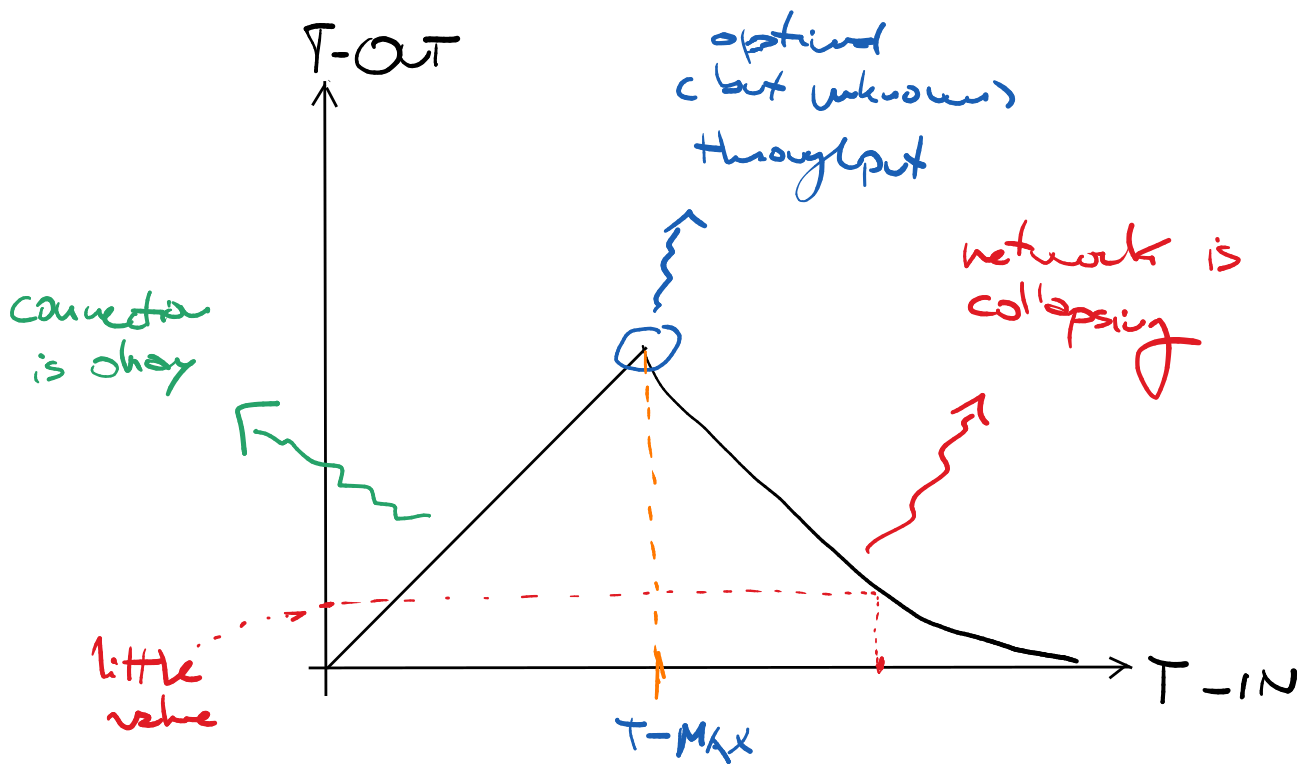
\includegraphics[ width=0.6\linewidth, height=\textheight, keepaspectratio]{./pics/tcp/networkCollapse.png}
    \caption{Network collapse after injecting a too-high throughput. Notice
        how injecting an even greater throughput will result in a \emph{lower}
        throughput.}
    \label{fig:networkCollapse}
\end{figure}


An excessive throughput \textbf{will} result in the following consequences:
\begin{itemize}
    \item packets exit \textbf{slower} than they entered;
    \item network's max sustainable throughput \texttt{T\_MAX} will
        \emph{collapse} \--- this fenomenon is called \textbf{network
        congestion};
    \item network \textbf{will need some time to remove its congestion},
        with even worse behavior in the case the unsustainable throughput is
        maintained for a longer time.
\end{itemize}

Intuitively, a network collapse happens because networks possess different
maximum speeds, a quality that cannot be appreciated by TCP, let alone for
networks \emph{different} than the one in which the device is sending data.

It is then up to the TCP layer to detect issues during path, and slow down
segments injection. Routers commonly have a mechanism for packet queuing, which
can be filled up, resulting in packet discarding. Such discarded packets will
need a retransmission, leading in even lower performance. New injected segments
and packets will increase the time for which the queue is dissolved.

\subsection{Congestion control}

\textbf{Congestion Control} algorithm takes into account the quality of the
network, allowing the sender to adapt to it instead of making it collapse.

Suppose the bound of flow control is so large that congestion control is
predominant (which means snd.congWin*MSS < snd.WinSize). A congestion control algorithm
could try do infer the maximum throughput by looking at the RTT and calculating
MSS/RTT < T\_MAX. However, this is unfeasible, since it requires too much
rounds and tentatives to be inferred.

A second issue is that the quantity T\_MAX \emph{varies during time}:
it depends on nominal throughput of networks and routers, and on
\textbf{competition} of different injected throughputs in the network.
Basically, the competition in the network is \emph{unpredictable} and
\emph{time-varying}, allowing no fixed\--value algorithm to work.

\subsubsection{Actual algorithm}

Congestion control algorithm has some important components,
\begin{enumerate}
    \item the \emph{slow start};
    \item the \emph{congestion avoidance};
    \item the \emph{fast retransmit};
    \item the \emph{fast recovery};
\end{enumerate}

each one with several variants and many parameters to be properly set. We will
see \emph{Tahoe} algorithm, but the most used one is the \emph{Reno}
algorithm.

The core idea of the TCP Congestion Control is to increase the so called
\textbf{congestion window}, a window size\--tracking variable, every time an
acknowledgement is received, while decreasing it a lot after a retransmission
timeout had expired, starting again from a lower speed. 

Initially, the
congestion window is set to a very low value: that is called \emph{the slow
start algorithm}. The slow start algorithm takes place if the congestion window
value is below a certain threshold, called \emph{SlowStartThreshold}; under the
slow start algorithm, the size of the congestion window increases very, very
quickly. After the congestion window size is above the threshold, the
\emph{congestion control algorithm} takes place, and makes the window increase
very slowly.

\begin{enumerate}
    \item The state variable \emph{CongestionWindow(t)} keeps track of a
        `virtual window' that is the actual quantity of data that can be
        injected through the network, and is initially set to a very small
        value (\emph{slow start principle}). Its value will increase whenever
        Acknowledgements are received in time \--- the network is assumed to be
        not congested. Upon retransmission (timeout expiration) the state
        variable is decreased a lot, and the network is assumed to be
        congested. 

    \item Another state variable, called \emph{SlowStartThreshold}, is
        a threshold under which \emph{CongestionWindow(t)} increases very fast,
        while above it the same state variable increases with a slower rate.
        Initial values of \emph{snd.congWin} and \emph{snd.ssThresh} are,
        respectively, $3$ MSS and $64KB$.

    \item Whenever an acknowledgement is received in time, the congestion
        window is increased. If the congestion window is lower than the
        threshold, increase fast with \textbf{slow start algorithm}; otherwise,
        increase slowly with \textbf{congestion avoidance} algorithm. The first
        will cause a fast growth in size of the window, the latter will instead
        produce a slower growth.

    \item Upon retransmission (timeout expiration), the congestion window is
        reset to MSS. Differently, the threshold is set to the maximum value between $2$
        MSS and \texttt{(snd.Next - snd.Ack)/2} \--- that is, the maximum value
        between the double of MSS and the half of the currently in-flight bytes. The
        assumption upon retransmission is that the network is congested: this
        behavior is inefficient in the case the network is not congested. Since
        \emph{many} concurrent causes may determine a packet loss \--- for
        instance, small RTO, network loss (e.g. WiFi) \--- one can end up with
        a congestion control algorithm forcing a slower pace of the network
        even though there is no actual congestion.

    \item The congestion window is increased according to the algorithm running at a given moment: 
        \begin{description}
            \item[Slow start algorithm] Congestion window is increased by +MSS
                whenever \textbf{any} in-time ACK is received. This is usually
                unaccurate, since the congestion window is usually
                \emph{doubled} after all segments have been received;
            \item [Congestion avoidance algorithm] Congestion window is
                increased by +MSS whenever \textbf{the last} in-time ACK is
                received, for all in-flight data.
        \end{description}
\end{enumerate}

The two algorithms increase the congestion window at \emph{much} different
speed. Slow start algorithm, despite its name, will \emph{double} the
congestion window each time an acknowledgement for all segments is received.
Congestion avoidance, instead, will increase the congestion window
\emph{linearly}, for which the window is increased by $1$ (single MSS) each
time an acknowledgement for all segments is received. The slow start will
provoke an exponential growth, while the congestion avoidance will provoke a
linear growth. 

\begin{figure}[hb]
    \centering
    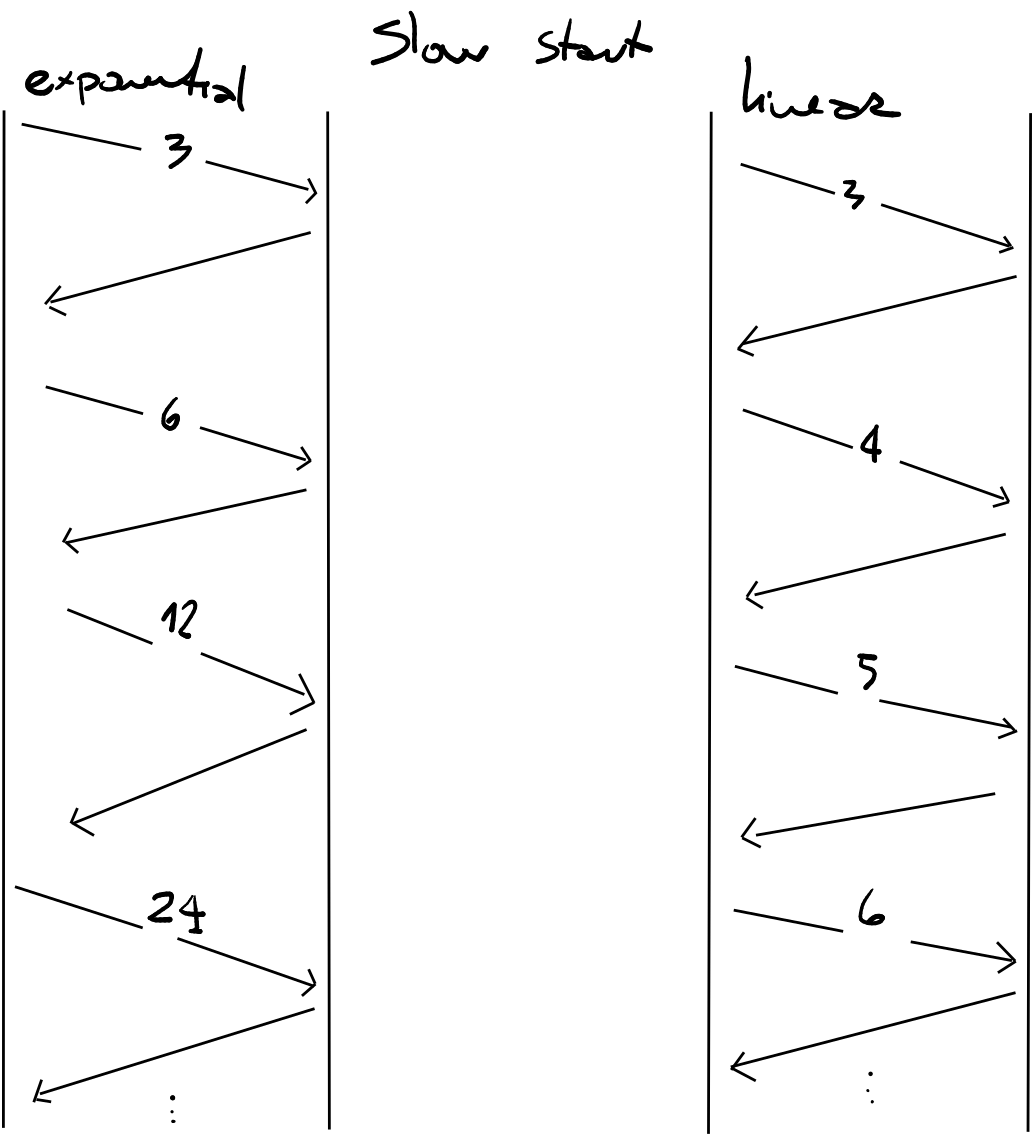
\includegraphics[ width=0.7\linewidth, height=\textheight, keepaspectratio]{./pics/tcp/slowStartTypes.png}
    \caption{The two kinds of slow start evolutions. At left, exponential, at
    right, linear.}
    \label{fig:slowStartTypes}
\end{figure}



\subsubsection{Congestion control and maximum throughput of the network}

What can happen on start?

Let's assume all segments are lost, and retransmission occurs after RTT (that
means, RTO is a good approximation of RTT). Let's also assume slow start
produces an exponential growth. Initial value of \emph{ssThresh\_start} is
$64KB$. Starting with threshold value below \texttt{T\_MAX}, slow start will
yield an exponential growth; after some time, congestion avoidance will enter,
a segment loss will occur and the congestion window will be reset to half the
\emph{ssThresh\_start} original value. 

Initial threshold above \texttt{T\_MAX}
will trigger a segment loss, and a reset of the threshold (without congestion
avoidance algorithm, that has not enough time to act). After the first segment
loss, threshold will be halved by setting it at half of the in-flight bytes,
and system will act as it started below the \texttt{T\_MAX} throughput. The
``exponential, linear, drop'' pattern will occur \emph{forever}, and the three
phases (slow start, congestion avoidance, loss detection) will happen one after
the other.

\begin{figure}[hb]
    \centering
    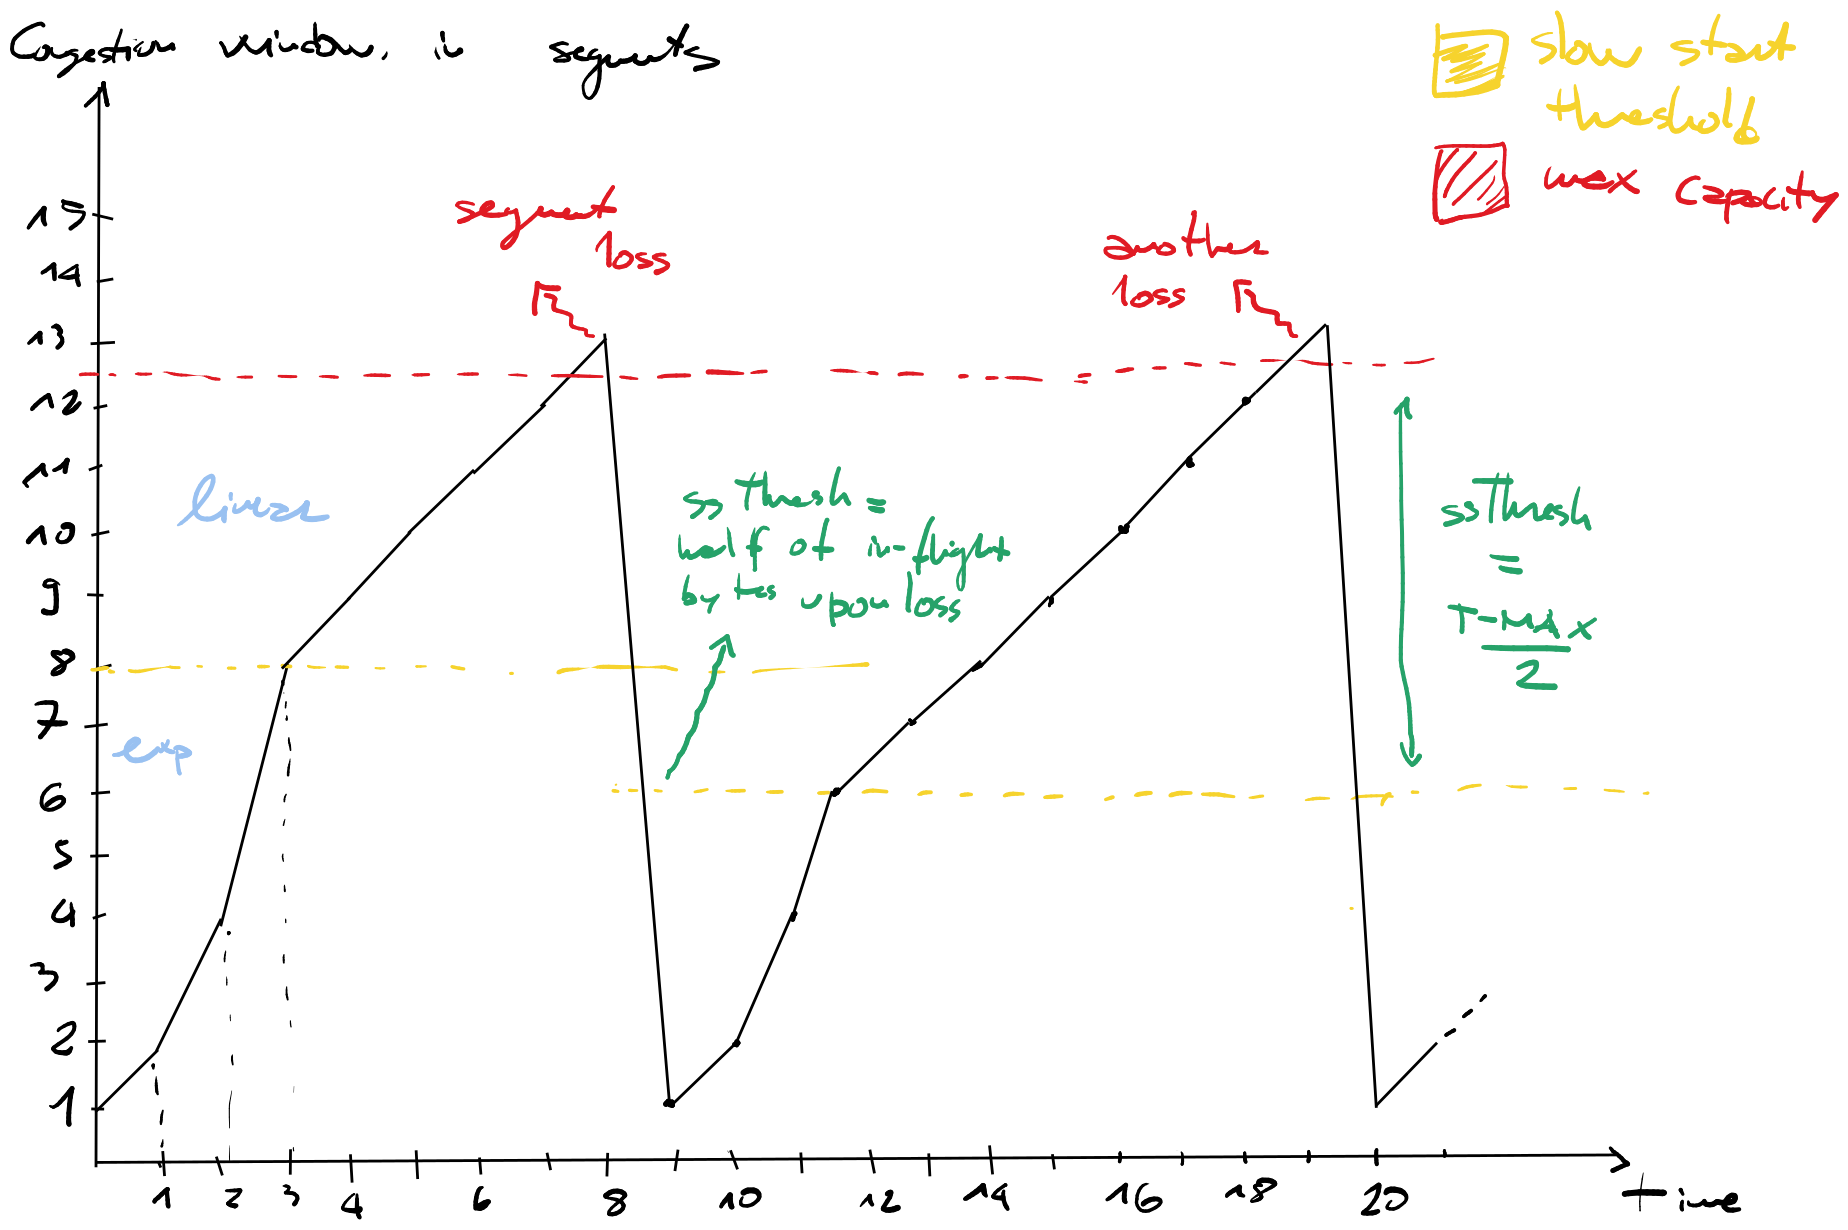
\includegraphics[ width=1.0\linewidth, height=\textheight, keepaspectratio]{./pics/tcp/congestionControl.png}
    \caption{Congestion control and its dynamics. The pattern indefinitely
    repeats.}
    \label{fig:congestionControl}
\end{figure}



\clearpage

With same assumptions as above, but with slow start provoking a \textbf{linear}
kind of growth, the pattern will be \emph{completely linear}, since no
exponential growth occurs. Basically, only the starting phase of each cycle
will be different. The end result in both patterns, however, is that the
average \texttt{T\_IN} value will be \textbf{much} smaller than \texttt{T\_MAX}:
the TCP congestion control cannot expoit internetwork capacity
efficiently. Injected throughput will always be lower than the maximum
possible: the consequence, is that the average throughput is lower than what
the network could sustain, however, this is very important in order to avoid
network collapse and congestion. 

There is a good reason for that: it is almost impossible to predict how the
network will behave. A network could host many devices, each one having
different demands, producing many kinds of traffic, each one with its own
\emph{volume}. The end result will be an unpredictable mess of network traffic.
The only way to adapt to this is to adopt an algorithm using a heuristic
behavior, that tries to adapt to the network as well as avoiding congestion the
most.

\subsubsection{Fast retransmit in a nutshell}

Suppose $K$ segements are transmitted in a burst, and a single segment among
them appears to be lost. Resetting the congestion window to its minimum value
is an inefficient move; since only a single segment of the row has been lost,
one could argue there is no need to drastically decrease the congestion window.

Another strategy could be \emph{waiting for a timeout before resetting the
congestion window}: the solution is inefficient too, since waiting before
retransmitting could lead to long breaks (how much to wait? how to estimate a
correct time interval?).

The \textbf{Fast retransmit} algorithm addresses precisely this kind of issue:
the solution is to retransmit \emph{immediately only} what appears to be the
missing segment, and decrease the window \emph{but not} to its minimum value
(that is, the maximum value between 2MSS and half of the current in-flight
bytes).

\subsubsection{Avoiding collapse of the network and the concept of fairness}

The congestion control slows down the network in order to assure both
\emph{collapse avoidance} and \emph{fairness}.

Intuitively, one would like to reach the maximum possible value for the
congestion window and the maximum throughput sustainable; however, both are
\textbf{unknown}. We can detect detect its value only after having injected an
excessive throughput, by detecing segment loss. However, whenever a segment loss occurs, the network is already congested. 

An aggressive slow down occurs
at each detection of segment loss, in order to prevent further collapsing of the
network. In fact, suppose many machines are injecting a throughput which is
closer to the maximum possible: in that case, if the network is congested,
\emph{it will require more time to return to its normal state}, because all
machines are insisting injecting throughputs close to unsustainable ones, and
removing congestion \textbf{will} require larger time. Basically, this is a
heuristic way to avoid congestion on a network where multiple machines are
using transmission resources altogether.

In the end, congestion control strives to ensure \textbf{fairness} with respect
to the other devices. Fairness is the tendency of each competing TCP connection
on a router to consume the same fraction of the router capacity. Each
connection, on average, will try to consume an equal fraction of router's
capacity. However, today's standard impose \textbf{node-level fairness}: this
means that each node should have the same amount of network capacity (thousands
of TCP connections can be opened at the same time from a single node). Note
that UDP connections \emph{do not} implement any flow or congestion control,
and transmit at full-speed: they are said to be `selfish'. 

Basically, the end goal of fairness is to grant anyone the same access of the
network, at the expense of your own networking speed (one could argue, however,
that if anyone tries to push as much traffic as possible in the network, no one
could be able to use the network, not even the same people that are pushing all
that massive traffic).

\subsubsection{Estimating the average throughput}

Some assumptions should be made in order to compute average throughput, given Congestion Control algorithm is running properly:
\begin{itemize}
    \item slow start has \emph{linear growth}. The congestion window starts
        from $1$ and goes up to $k+1$;
    \item \texttt{T\_MAX} is constant and in between $K\cdot MSS$
        and$(K+1)\cdot MSS$;
    \item \emph{all} segments are lost at once (no wild retransmissions);
    \item all segments are received up to $k$-th round; segments in round
        $k+1$-th are all lost at once;
\end{itemize}

The \emph{average throughput} that is injected is the average number of bytes in each
pattern, divided by $(K + 1)\cdot RTT$. The number of bytes in each pattern is
equal to MSS * number of segments in each pattern \-- since we are assuming a
linear growth, the segments are increasing linearly up to $k+1$, that means the
number of segments belonging to a pattern is $\frac{k \cdot (k + 1)}{2}$;
hence, the \emph{average throughput formula} is

$$A_t = \frac{MSS\cdot \frac{K(K+1)}{2}}{(K+1)\cdot RTT} = \frac{MSS\cdot
K/2}{RTT}.$$ 

Thus, the injected throughput is the same one would obtain by
having a \emph{constant window} of $K/2 \cdot MSS$ size \--- on average and
under ideal conditions, one can only get \textbf{half} of the maximum network
throughput.

Slow start in exponential fashion makes this calculation quite more complex,
but we will genuinely assume a linear growth in all our calculations, to make
them simpler.

\subsubsection{Idle connections}

Another important scenario that has not been disclosed yet is about \emph{not
transmitting data after many RTTs}, the case of \emph{idle connections}. The
basic idea is to reset the values of congestion window and slow start threshold
after a timeout expired (RTO).

Without a reset, one would use the last values that were determined by the
congestion control algorithm. In order to avoid bad performance, the sender
\textbf{resets both congestion window and slow start threshold} after a
timeout. Basically, by resetting the connection state regarding previously
achieved speed, the approach tries to be very pessimistic and conservative, in
order to avoid any kind of congestion in the network.

\subsection{Interaction between flow control and congestion control}

The interaction between the two TCP control systems is not straightforward.
After connection opening, the bound imposed by congestion control is
\emph{much} tighter than the flow control one (2-4 MSS instead of $64KB$).

Hence, at the beginning the network \emph{will follow congestion control}'s
dictated bounds: data transfer begins slowly.

After connection opening (steady-state), there are two possible cases:
\begin{itemize}
    \item \texttt{T-MAX > T-FLOW-CONTROL} \--- when the maximum network
        throughput is greater than the maximum flow control throughput: in this
        case, the bottleneck is the \textbf{receiver's capacity}. The steady
        state throughput will be $\frac{M\cdot MSS}{RTT}$, while its connection
        opening transient throughput will be half of that value, that is
        $\frac{M \cdot MSS}{2RTT}$. What happens here is that there is a
        steady-state with a fixed value due to the flow control algorithm,
        while before reaching it and during the opening phase the speed
        increased following congestion control (slow start or congestion
        avoidance depending on how the slow start threshold has been initially
        selected);
    \item \texttt{T-MAX < T-FLOW-CONTROL} \--- when the maximum network
        throughput is lower than the maximum flow control throughput: in this
        other case, the bottleneck is the \textbf{internetwork}, and congestion
        window will go up and down, never reaching the value corresponding to
        the receiver's buffer size. The steady state throughput will be
        $\frac{K\cdot MSS}{2MSS}$. Basically, in this case the flow control
        never occurs, both receivers will never reach their full speed and the
        real culprit would be the internetwork.
\end{itemize}

Since the steady state during congestion control is variable and corresponds to
half of the actual internetwork speed, reaching a flow control steady state is
much more desirable, especially when the flow control window size is set
slightly below the maximum throughput. However, the exact \texttt{T\_MAX} value
is unknown and varies overtime, therefore it is impossible to reach such an
ideal scenario.


\subsubsection{Congestion control variants}

Many variants of Congestion control have been developed. In particolar, there
are many families for different use-cases:
\begin{description}
    \item[congestion collapse] this class attempts to increase the average T-IN
        upon congestion collapse in a standard, wired internetwork connection;
    \item[wireless] this class strives to optimize correct non-wired environments, with algorithms tailored to environments with high network loss;
    \item [high-speed] this class is tailored to sustain very-high bandwidth
        connections (e.g. backbones), with \emph{high bandwidth-delay product}.
\end{description}

The latter is the case of \emph{backbones}, with very-high bandwidth-delay
product \--- those are all the networks that, if TCP is left as default, will
lead to several minutes of connection start and gigabytes of data exchanged for
the sole goal of bringing the connection to full-speed! In order to optimize
them, several variants of TCP have been developed.

As an example, suppose a sustainable throughput $T_{MAX} = K \cdot MSS /
RTT$, and suppose the length of the first initialization period be $t_{init} =
K \cdot RTT$. Solving in $K$ leads to $$t_{init} = \frac{T_{MAX} \cdot
RTT^2}{MSS}.$$ By looking at the formula, one recognizes that the initial time
has a squared dependency over round-trip time, a direct proportionality over
$T_{MAX}$ and is inversely proportional to MSS. In all connections where both
RTT and $T_{MAX}$ are large or extremely large, the initialization time could
become relevant as well as the sheer quantity of the data that is needed (more
than $3$ minutes of transient, more than 100GB transmitted). For this reason,
variants of TCP for backbones are mandatory.

The following Table~\ref{tab:warmUp} sums up the values for some kinds of
connections, in the case of congestion control only.

\begin{table}[ht]
\centering
\begin{tabular}{r|cccc}
    & \textbf{\makecell{10Mb/s\\ 10ms RTT}} & \textbf{\makecell{10Mb/s\\ 2ms RTT}} & \textbf{\makecell{1Gb/s\\ 10ms RTT}} & \textbf{\makecell{10Gb/s\\ 10ms RTT}} \\
    \hline
    \textbf{MSS} & 536B & 536B & 536B & 536B \\
    \\
    \textbf{Maximum congWin} & 23 & 5 & 2332 & 23321 \\
    \\
    \textbf{\makecell{Congestion control\\ throughput (Mb/s)}} & 5 & 5 & 500 & 5000 \\
    \\
    \textbf{Transient} & 0.2s & $\sim$0.0s & 23.3s & 3.9m \\
    \\
    \textbf{Transmitted data} & 145.8 KB & 5.8 KB & 1475.6 MB & 145.76 GB
\end{tabular}
\caption{Warm up time for different kinds of connections, using the standard
TCP protocol with a standard congestion control. Notice the sheer number of
seconds required to warm up a 10-gigabit network and the unsustainable quantity
of transferred data when adopting the standard TCP protocol.}\label{tab:warmUp}
\end{table}
\bigskip

\subsubsection{Estimating the data exchange time}

Let \texttt{T\_MAX} be known and let $M$ the flow control window size be known
as well; $B$ bytes should be sent. To estimate the time of the entire data
exchange, a solution could be to first estimate the maximum number of bytes in
the transient phase, that is $$N = MSS \cdot [(\frac{M \cdot (M + 1)}{2}) -
3];$$ if the obtained quantity $N > B$, then the entire data exchange occurs
under congestion control. Otherwise, a portion $B - N$ of the bytes would fall
under one of the two possible steady states, depending on the relationship
between the maximum throughput of the network \texttt{T\_MAX}, and the window
size $M \cdot MSS$.

Notably, throughput in congestion control cannot be assumed to be exactly
$\frac{T\_MAX}{2}$ -- in fact, that is the average value over \emph{multiple}
periods, possibly many of them. In the case of a small value $B$ to delivery,
one could not have enough periods to assume the average throughput is the half
of the maximum throughput of the network.

Knowing \texttt{T\_FC} in place of $M$, one can easily find a solution by the
same means as above. However, one should take in account that in order to
understand whether the steady state lies in congestion control or in flow
control, one has to confront the throughputs so that only in the case of
$T\_MAX < T\_FC$ the steady state occurs under congestion control.

\subsection{Reliability of TCP}

TCP is a \textbf{reliable} protocol. The reliability in TCP only means that
exchanged data are received, in order, and with no duplicates.

A common misconception about TCP is that the \texttt{send()} system call
provides both delivery and reliability. Unfortunately, the \texttt{send()} call
only guarantees that the data has been handed to the underlying operating
system, without being able to tell whether the data has been successfully
delivered or not. In order to do so and achieve reliability, the application
must ask for data by invoking \texttt{receive()} -- the \texttt{receive()} call
will check whether there is a segment with a correct \texttt{ACK} or not.

Application layer invoking \texttt{send()} does not know how many bytes are
received by the other side of the connection. The \texttt{send()} call may
complete with no error, but no byte could have been transmitted \--- there is
no way to know how many packages are actually delivered to the other party.

Suppose the \texttt{send()} invocation ends with an error message.
Upon an error taken during the $n+1$-th send invocation, there is no way to
know if previous messages were actually delivered or not. Despite TCP being
reliable, there is \textbf{no guarantee} that messages up to $n$-th were
delivered and transmitted, since the error message for \texttt{send()} call
simply means there have been a failure in the TCP protocol, and data cannot be
handed over to the operating system.

The correct reasoning is that all bytes \emph{up to} $k$ are correctly
delivered, but one cannot know the exact value of $k$. 

Regarding bytes delivered to the application level at the other end, bytes were
received by TCP layer up to $k$ but probably $k - k'$ bytes \emph{are still to
be delivered to the application}. This means only a portion of them, $k'$, have
been delivered. Both $k$ and $k'$ are \emph{unknown}.

Hence, there is no exact possible reasoning on TCP when it comes to a
\texttt{send()} invocation, since application should call \texttt{receive()}
instead to be sure all the data up to $k$ has ben received.

Only after \emph{receive} call, with all ACK correctly received, one can be
sure that all previous data have been successfully delivered. 

Upon \texttt{receive()} or \texttt{send()} error, one \emph{cannot tell
anything about the previous \texttt{send()} invocations up to that
\texttt{receive()} call}, since there is no clue whether the packet has been
received correctly or not.

Any of these scenarios might be the reason for a \texttt{send()} failure:
\begin{itemize}
    \item \emph{not received}: packet never received by the partner;
    \item \emph{not delivered}: packet arrived, but partner crashed before
        reply;
    \item \emph{delivered}: packet delivered, but not reaching, connection is
        broken.
\end{itemize}

All these scenarios must be handled differently and correctly. Response to
failure should always be a correct failure handling and proper recovery from
damage, no matter its kind. Typical examples of error handling are:
\begin{enumerate}
	\item first, take an error;
    \item repeat the message;
    \item wait some time;
    \item send request again;
    \item do until receiving a response.
\end{enumerate}

However, this approach is often wrong. In fact, the party is repeating the same
request over and over, possibly producing an effect multiple times.

When dealing with financial transactions, same requests can be performed
multiple times, and lead to catastrofic errors and wrong operations. Only read
operations can be handled this way effectively.


\section{Opening a TCP connection}

\subsection{Sequence numbers initialization}

Opening a TCP connection involves the decision of the \textbf{starting sequence
numbers}, whose value is not necessarily set to $0$.

Upon connection opening, since they are not set to zero, each of the two sides
should agree to their initial sequence numbers. The ideal starting point is
that every \texttt{snd} pointer should be set to the same value, as well as the
other party's \texttt{rcv} buffer. 

A first idea could be to simply send initial
segments in which \texttt{snd.Next} are specified in header. Special segments
could carry a flag that denotes a connection request (from the client) and \texttt{OK}
(from the server). Both parties will set their initial \texttt{rcv} pointers
accordingly to the value read in the header from the other party. 

In reality, this first implementation suffers from many issues:
\begin{itemize}
    \item delayed duplicates from client may be received after a long time \---
        the server might uncorrectly believe another connection request is
        coming from the client (since there are port numbers, however, the new
        connection will be opened only in case the previous one has been
        closed);
    \item delayed duplicates from server may be received after a long time \---
        this way, an opening with wrong sequence numbers may occur. In fact,
        suppose a server initial \texttt{snd.Next} number is equal to $63$ and
        sent via a delayed segment. Now, if the server has sent another segment
        (which has not been delayed) with, let's say, \texttt{snd.Next} equal
        to $91$, the client would believe the server has chosen $91$ as the
        starting sequence number. This is not correct, indeed.
\end{itemize}

The solution to the above problems, in which delayed packets may be
undistinguishable from not delayed ones, is the ``\emph{cross your fingers}''
approach. Both machines \emph{assume} that a predefined, \emph{maximum segment
lifetime} exist, after which segments cannot exist. 

 The lifetime in question is named \textbf{Maximum Segment Lifetime (MSL)}, and
 it is arbitrarily set to $2 min$ ($120s$). After such MSL time passed, the
 machine simply assumes that the missing segment will never reach it. This is,
 in reality, wrong: IP do not have concept of \emph{time}, and packets are
 discarded only based off their number of \emph{hops}. Since the assumption
 does not match reality, the algorithm execution does not provide any
 guarantees --- it does, however, guarantee that no wrong duplicates may
 possibly reach the other endpoint.


\subsubsection{The three-way handshake protocol}

The sequence numbers are generated by the \textbf{ISN-generator} (initial
sequence number generator), a $32$-bit counter increased every $4\mu s$, even
when the connection is switched off. Overflow will eventually happen every $4$ to $5$
hours. The generator is used to generate an initial sequence number from its
current value; a sequence number can be used again after at least $4$ hours,
after the ISN-generator will overflow.
\begin{figure}[b]
    \centering
    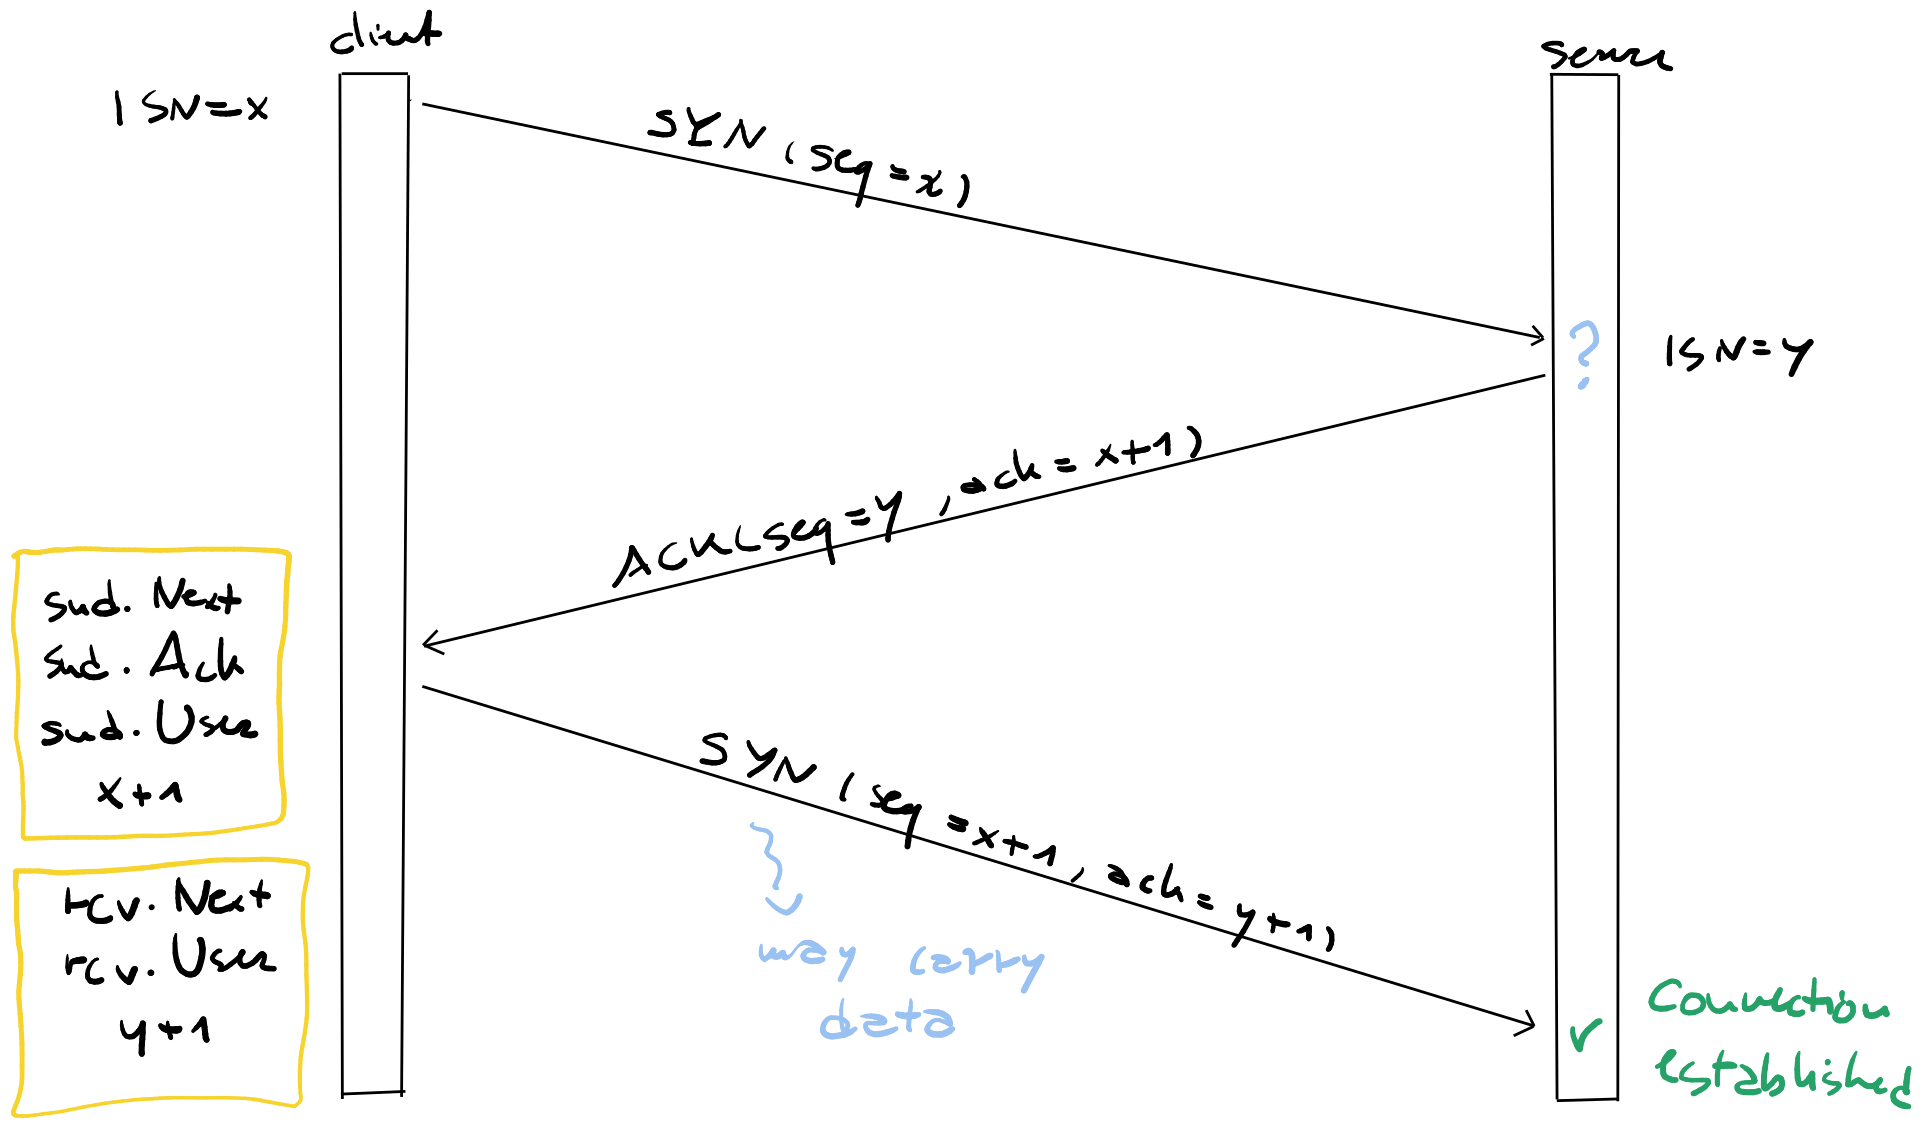
\includegraphics[ width=1.0\linewidth, height=\textheight, keepaspectratio]{./pics/tcp/threeWayHandshake.png}
    \caption{The three-way handshake.}
    \label{fig:threeWayHandshake}
\end{figure}

Upon connection opening, the initial sequence number will be obtained by
querying the ISN-generator.

The three-way handshake protocol (Figure~\ref{fig:threeWayHandshake} will begin
with sequence number initialization, whose value has been obtained from the
ISN-generator (suppose it's $x$), and send a \texttt{SYN(seq=x)}\footnote{SYN bit is a
flag in TCP header that is always zero, except in the first and second
segments, and it is used only for requesting connections.} packet to the
server. The latter will answer with a package such as \texttt{SYN(SEQ=y,
ACK=x+1)}, signaling both server's initial sequence number and that it has been
acknowledged bytes up to $x$, and it is ready to receive the next (actually the
first) byte.

The client will then respond with a second
message, containing data and having sequence and acknowledgement numbers
\texttt{(SEQ=x+1, ACK=y+1)}, showing that it is ready to receive the first byte
after $y$ as well; now, connection has been established and both parties will
assume the connection is successfully opened. 

The client side will be sure that no delayed duplicates are coming, otherwise
$x$ would have come from a connection which has been opened more than $4$ hours
ago! The same reasoning happens from the server side: any delayed duplicate
should have been traveling for more than $4$ hours, which is almost impossible
to happen. 

This protocol even protects in the case \emph{old duplicates} are delivered to
a server: in that case, the server will open a connection since the request looks legitimate. However, when the client receives the packet from the server \--- for
something they did not request at all \--- it will respond with a
\texttt{REJECT} packet\footnote{\texttt{RST} is a header flag as well as
\texttt{SYN}, and it is used only to reject connections.}. The server will
finally answer with a \texttt{REJECT(ACK=y+1)} to signal it has correctly
acknowledged the request to close the connection.

A very unlucky case is where the server receives two delayed duplicates, one
coming to open a connection and the other one just after the server sent its
\texttt{ACK}; however, there is little to no chance that the ACK values are
correct (and, in that case, it would have traveled for more than $4$ hours,
much more than MSL value of 2 minutes). In fact, in those cases, rogue packets
from a client would contain \texttt{CR(seq = x)} and \texttt{DATA(seq=x+1,
ack=z)}, with the server expecting an acknowledged sequence number \texttt{y}.
The same goes if the server receives a \texttt{REJECT} (it cannot be a
duplicate). The mechanism is shown in Figure~\ref{fig:threeWHduplicates}.

\begin{figure}[b]
    \centering
    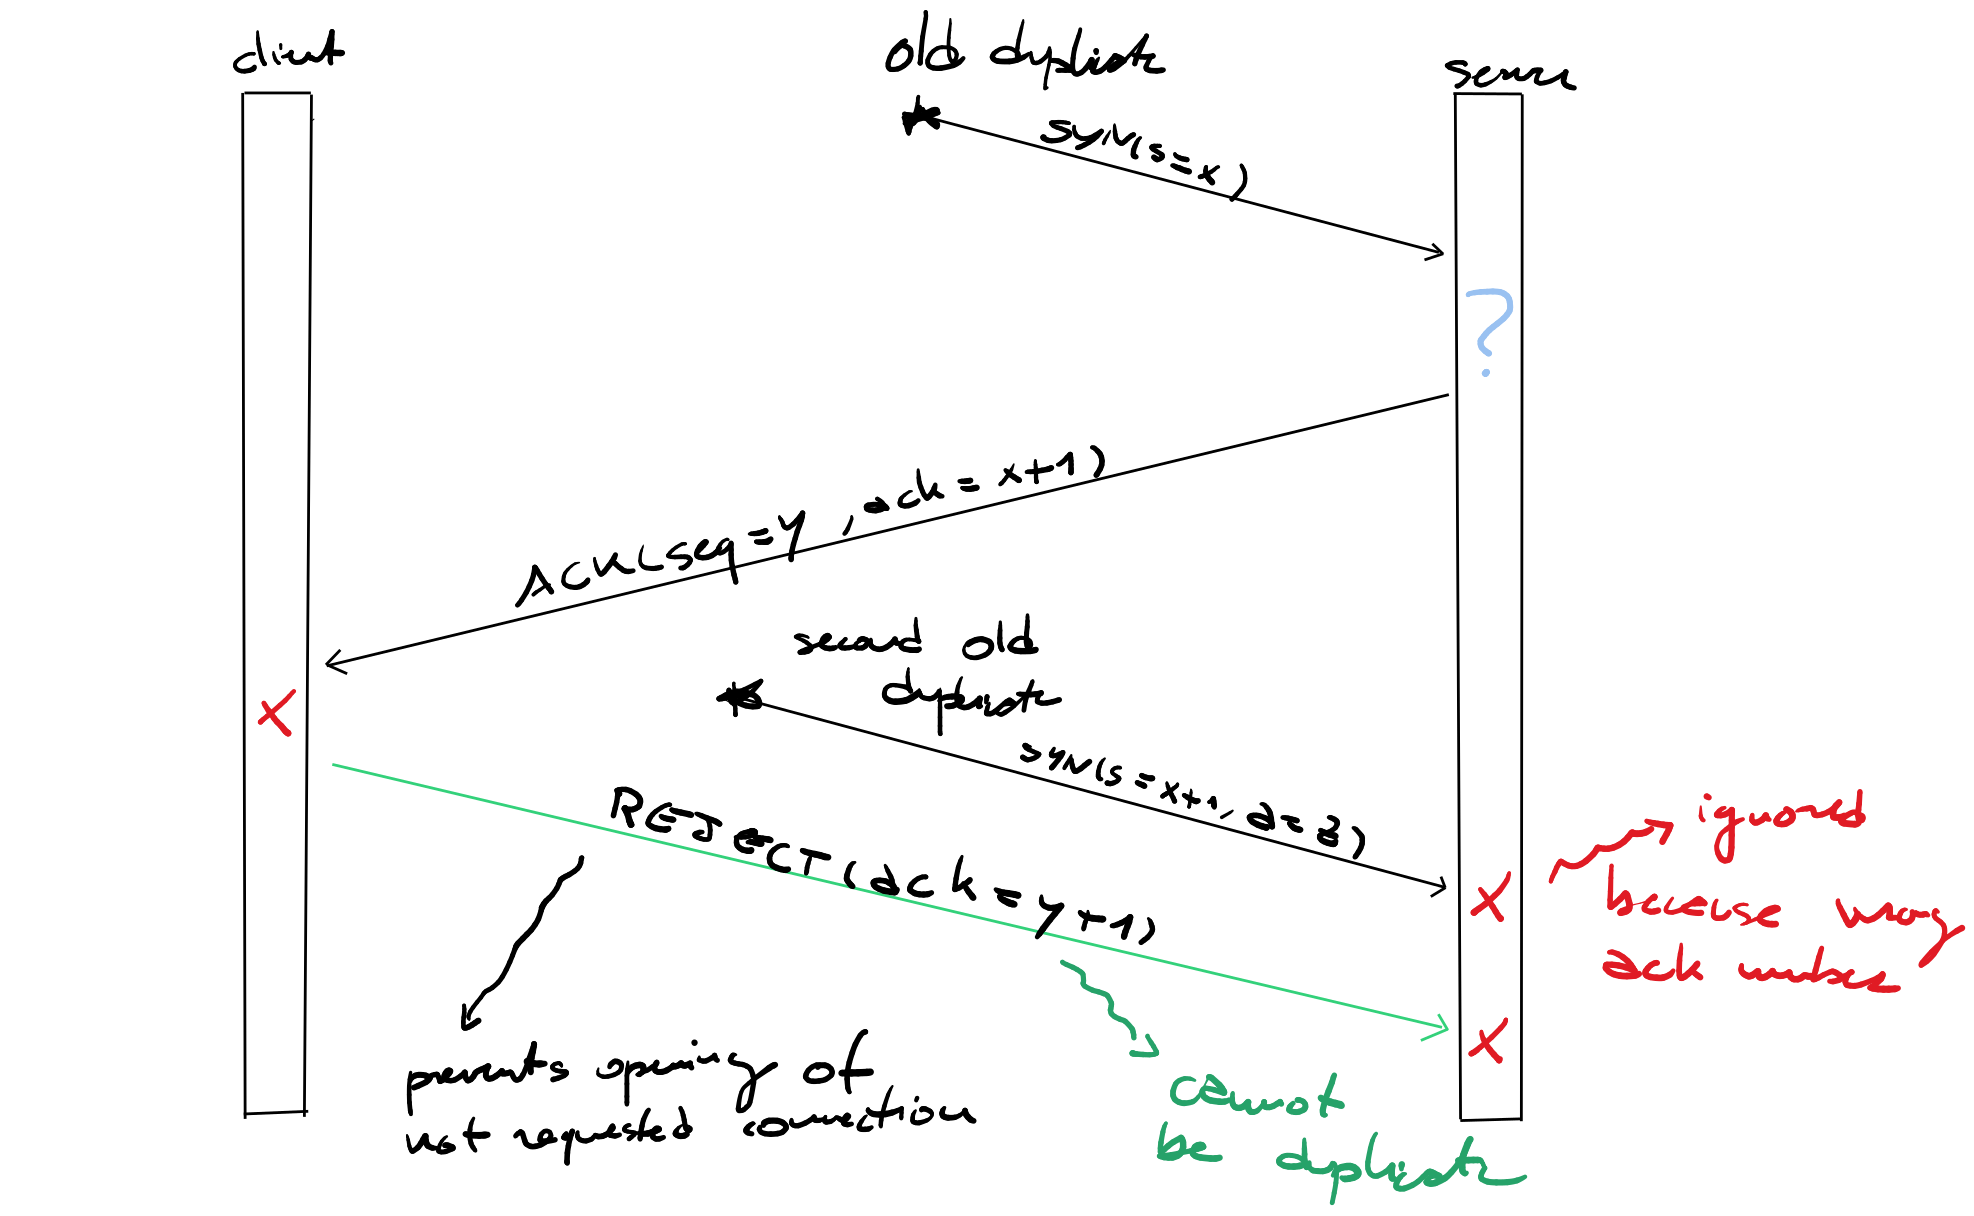
\includegraphics[ width=1.0\linewidth, height=\textheight, keepaspectratio]{./pics/tcp/threeWHduplicates.png}
    \caption{Possible errors in TCP handshake. The TCP protocol and its
    sequence number system is designed to avoid unsolicited connection opening,
preventing the server to waste resources with no reason.}
    \label{fig:threeWHduplicates}
\end{figure}



As we have already said, \texttt{RST} flags are used to reset a connection, or
close an unwanted one. \texttt{RST} segments should be sent in two cases,
\begin{itemize}
    \item unexpected \texttt{rcv-seqnum} in 3-way handshake;
    \item received segment for closed connection;
\end{itemize}
and in those cases, the \texttt{RST} segment is sent with the sequence number that is
expected by the peer.

In case the \texttt{RST} packet is legit (that is, when it carries the sequence number
the machine expects), then \textbf{close} the connection and \textbf{ignore}
\texttt{rcv-segment}.

\subsection{Interface between 3-way handshake and application layer}

To open a connection, application layer just requests TCP to open a connection.
The TCP layer will handle the connection opening with the appropriate system
calls, with the protocol as described above.
The system calls in sequence are

\begin{itemize}
	\item \texttt{socket};
    \item \texttt{bind};
    \item \texttt{listen(num, ...};
    \item \texttt{accept}.
\end{itemize}

System call \emph{listen} has a \emph{num} in argument that tells \emph{how many
connections can be queued}, that is, the number of incoming \texttt{SYN} segments that
should be queued before opening connections. Until \texttt{listen} call has
been invoked, no connection can be opened and the server will respond with
\texttt{RST}. Up to \emph{num} \texttt{SYN} segments can be accepted at the
same time \emph{before} invocation of accept and delivery of \texttt{SYN-ACK}
packages. For instance, if \texttt{num=5}, the server will wait for $5$
connection requests before actually answering to the client and opening the
connections.

Closing a connection is done with the \texttt{FIN} flag. It is handled the same
way as \texttt{SYN} is, and where one party wants to close connection, sets
\texttt{FIN} flag to $1$ and the other party will respond with a \texttt{FIN}
flag to $1$ as well.

This protocol can be abused to block a server with little to no effort. Attacks
whose goal is to prevent the target working are called \textbf{Denial of
Service} attack. An example of DoS attack is the \textbf{SYN-flood} attack.

The idea is to keep sending \texttt{SYN} segments so that server queue \emph{is
always full}: the effect will be that legitimate \texttt{SYN} requests from
legitimate clients will be discarded. Some variants even hide the
\texttt{IP-src} by modifying it, in order to hide attack origin. This way, it
is impossible for a defender to prevent the SYN-flood by blacklisting IP
addresses. Moreover, \texttt{SYN-ACK}s responses will be delivered to (fake)
IP-src address.

SYN-flood attacks are very hard to detect and very cheap to operate.
Indeed, randomly forging \texttt{IP-src} addresses makes almost impossible to
filter them out with a firewall. SYN-flood attacks are also cheap: for $128$
opened connections every $3$ minutes, only $128\cdot 40 = 5120B \mbox{ every }
180s = 228 bps$ bytes are needed to the attacker to forge necessary packets. To
forge $1280$ connections, $1280\cdot 40 = 51200B \mbox{ every } 3 m = 6826bps.$
A small cost of sending a packet causes the listener to force a listening to a
connection, a \textbf{much} higher cost. 

By designing a new protocol, one would likely avoid spending resources upon the
first \texttt{SYN}, by operating \emph{statelessly} until the initiation can
demonstrate its legitimacy. However, a new protocol is almost impossible to
design, since existing network architectures cannot simply be replaced.


\chapter{Threat model}

\section{Understanding threat model}

TCP offers \textbf{no authentication mechanism}. It means that if, for example, the
address has been maliciously altered in DNS, a connection can be opened to the
attacker's service rather than to the legitimate one and the client would not
notice the difference. Network attacker may be in control of the router, too
\--- he might be capable of switching DNS requests and respond with fake
responses.

TCP offers \textbf{no integrity mechanism} either. A network attacker might
change what the machine sends and receives \--- a communication may be altered
by an entity that acts in between the two legitimate parties. Fortunately, an
improved version of TCP, \textbf{TLS (Transport Layer Security)}, is available.
It works by acting on top of TCP, and uses \emph{cryptography} to provide
integrity to protect the message and offers a strong authentication mechanism.

However, TSL can still be compromised: Suppose in fact the client has been
infected by a \emph{malware}\footnote{A \emph{malware} is a malicious software,
secretly installed by the attacker and against the user's consent, to perform
ill--intentioned behavior} --- then the attacker can control the client's
behavior from remote, for example modifying web pages, opening connections,
attempting privilege escalation\footnote{\emph{Privilege escalation} is a
technique in which an attacker that has gained unprivileged access to the
machine tries to obtain super--privileged access by means of exploits,
vulnerabilities and by other techniques. For instance, an attacker could try to
obtain \emph{root access} and root privileges to perform anything he wants on
the machine.} on the machine. In this case, TLS does not guarantee secrecy,
integrity, authentication.

An crucial question arises: \emph{is then TLS vulnerable and therefore pointless?}

Basically, it all depends on \textbf{threat model}. A threat model is the set
of actions that \emph{we assume the attacker can execute}. One makes an
\emph{hypothesis} on the set of attacks that are possible, and then it reasons
accordingly. In fact, reasoning about security of a system without a well-posed
threat model makes no sense at all, because an attacker that doesn't have a
predefined set of attacks and can do anything is an attacker it is impossible
to defend against. That said, a \emph{real attacker} may not be confined in a
single, limited, threat model, because it both may be modeled unaccurately and
it may be unpredictable.

An important remark is that all protections in software are designed with a
specified threat model in mind. They do not work outside their threat model
which they are based on, and for this reason software should be chosen
accordingly. Both protections and possible kinds of attackers are important to
be established before acting, in order to minimize expenses, maximize defense
capabilities, and increase the chance an attacker is successfully repelled.

Important questions when dealing with attackers are the following ones, 

\bigskip
\setsansfont{Source Sans 3}
\begin{quote}
\begin{center}
    \sffamily {What's the \emph{threat model} for that specific attack technique?

\bigskip
    What's the \emph{least pessimism} required in order to execute an attack?

\bigskip
    What's the \emph{best software} in terms of \emph{cost}, \emph{defensive
    capabilities} and \emph{chance to be attacked} that should be used to
defend to a given attack?}
\end{center}
\end{quote}
\bigskip
\setsansfont{Source Serif 4 Display}

Typical threat models involve the following scenarios, in increasing pessimism:
\begin{itemize}
    \item \textbf{Network attacker} \--- the attacker can only operate in the
        network. He is able to observe and communicate. DoS (Denial of Service)
        and MITM (Man in the Middle) attacks are usually what a network
        attacker can do;
    \item \textbf{Compromised endpoint} \--- the attacker compromised a node in
        the network with a malware. That node is fully compromised and should be
        considered not trusted;
    \item \textbf{Physical access} \--- the attacker obtained physical access to an
        endpoint. Regardless of the fact a machine is already infected or not,
        physical access grants much more privileges than the above threat models,
        for instance it can compromise much more easily an endpoint or can
        install devices that are physically capable of acting as man in the
        middle;
    \item \textbf{Evil maid} \--- a \emph{variant} of both \emph{physical
        access} and \emph{insider} threat models in which an person that has
        frequent physical access to a machine is instructed to perform
        operations on the device. An evil maid has no access on supply chain or
        organization internals, though;
    \item \textbf{Insider/Supply chain} \--- this very dangerous attacker has
        access to portion of the \emph{software supply chain}, for instance it
        can manipulate software libraries the main software depends on,
        infrastructure on which the software development occurs, and so on. In
        the case of the insider, it also has access to the internal
        communications and is able to actively spy the organization he is into.
\end{itemize}

The TLS (and by extension, the HTTPS protocol) grants \emph{secrecy},
\emph{integrity} and \emph{authentication} only for a network attacker--based
threat model. Outside that model, TLS and HTTPS offer no guarantee of
protection.

\subsection{Choosing the defenses}

Threat models are also useful to define from which kinds of attacks one should
defend, from which ones one cannot defend and should act accordingly, and from
which ones one simply has to ``cross his fingers'' (do nothing).

The first category of attacks should be treated with proper software that
offers protection against a well--defined threat model. Outside that model, the
software should be considered useless and the system that it protects is
compromised and not anymore trusted. This category of attacks is rather
frequent, doesn't cost too much, and poses immediate danger to the activity of
the organization. 

The second category, whose best defense is \emph{damage compensation}, is the
category of attacks that are not very frequent and whose relative defensive
mechanisms cost too much to be economically viable and sustainable for the
defending organization. In these cases the organization simply prepares for
damage mitigation, with strategies such as \emph{data backups}, \emph{backups
of systems} and by other means.

The third category is both rare and costly. These kinds of attacks are very
dangerous, but occur extremely rarely. It is therefore rational to simply allow
this kind of risk to happen, without taking any countermeasure in account.

An crucial remark is that for \emph{choosing the defenses}, it is not important
\textbf{how} an attacker has managed to operate an attack, and it suffices to
know the specific threat model and attack set an attacker is able to conduct.
For \emph{assessing likelihood} of a threat model, in order to decide the
actions to take, it suffices to know how an attacker has been able to achieve a
certain attack capability.

In fact, the details on how an attack works and how it is only necessary to
find and determine the cause of a given vulnerability or exploit.

The first step of a defender should be to determine a threat model by looking
at how simple is for an attacker to achieve a certain specific attack. The next
step is to determine the best defenses \emph{given} a threat model.


\subsection{The network attacker threat model}

The \emph{network attacker} threat model is implicitly assumed in this book. A
network attacker can only operate in the network, by communicating, observing
and altering existing traffic. An attacker of this kind cannot act on the
endpoints.

The implicit assumptions are that everything on the endpoints is perfectly
implemented, operated and maintained -- this means that there are no
vulnerabilities, no exploits, and no obvious mistakes by the system
administrator. Software is perfectly maintained as well. No mistakes are
allowed, no remote code execution, no vulnerability, no mistakes from the
users, in cryptography, protocols and communication, and operating systems.

These kind of assumptions are important to confine the attacker to the network
threat model; otherwise, an attacker could be able to infect an endpoint,
upgrading the threat model to the \emph{compromised endpoint} threat
model.

The key defensive tool against a network attacker is \textbf{cryptography}.
Cryptography allows both \emph{secrecy} and \emph{integrity}, and by means of a
structured trust system it allows \emph{authentication} as well. All of these
protocols make use of cryptography:
\begin{itemize}
    \item TLS and HTTPS;
    \item Kerberos;
    \item Windows Active Directory;
    \item OAuth (SPID);
    \item SSH;
    \item IPSec;
    \item Legally binding digital signature;
    \item WhatsApp, Signal, Telegram;
    \item and so on.
\end{itemize}

Examples of possible attacks a network attacker is capable of are listed below,
\begin{itemize}
    \item \textbf{DNS Spoofing} -- a DNS attack in which an attacker modifies
        the IP address (and the ID in header) contained in the response to a
        DNS query, in order to hijack a client to an attacker controlled
        server, and act as man in the middle, or showing a perfect copy of
        another website. Windows systems are particularly vulnerable to this
        kind of attack, since by default they prefer any IPv6 server and
        happily substitute the preconfigured IPv4 server upon a malicious
        packet containing new instructions arrive;
    \item \textbf{ARP Spoofing} -- fake responses crafted by an attacker, whose
        goal is to make a device change its default gateway to an attacker's
        controlled device, so that it can act as man in the middle. Open WiFi
        is vulnerable to this kind of attacks;
    \item \textbf{BGP Spoofing} -- highly--skilled attack in which an attacker
        manages to alter the routing of the internet, so that it can direct
        traffic to different places. Border Gateway Protocol messages are not
        authenticated; Autonomous Systems can claim ownership of any IP
        address;
    \item \textbf{Dishonest system administrators} can act as man in the middle;
    \item \textbf{Judicial authorities} or \textbf{intelligence agencies}
        possess huge available resources, and can force organizations, internet
        nodes and system administrator to act as man in the middle.
\end{itemize}


\section{Attacking TCP connections}

A legitimate threat model for a TCP connection is the network attacker threat
model. A network attacker can observe, communicate and alter traffic by acting
as man in the middle in all communications between two endpoints.

The first model of the network attacker that strives to control a TCP connection
is the \textbf{on--path attacker}. The on--path attacker is able to read
integrally the communication between the two endpoints, and can act as man in
the middle.

The objective of the first kind of attack we will encounter is the \emph{client
impersonation} in a TCP connection between a client and a server. The server
will see the IP of the client at the other end of the communication, whilst
packets are actually sent and received by the attacker.

There are three possible ways to perform such an attack:
\begin{enumerate}
    \item \textbf{Opening a connection} and impersonating the client's IP
        address;
    \item \textbf{Injecting some data} in an already opened connection;
    \item \textbf{Closing a connection} already running.
\end{enumerate}

In the second method, the attacker only injects \emph{part} of the
communication, and represents a less pessimistic approach, in which the attack
does not manipulate the communication and can only inject data. The third
method is the more optimistic one, with the attacker only capable of closing an
existing connection in order to perform some kind of denial of service.

All three attacks are trivially feasible, with an attacker able to act as man
in the middle. In the first case, the attacker is able to intercept an opening
connection, and starts handshake with the server, opening a connection.

An on--path network attacker is able to intercept all segments. In particular,
such attacker is interested in obtaining sequence numbers, so that it can
successfully replicate the connection state, inject data, and manipulate
correctly the connection by means of forged segments with correct sequence
number.

Data injection by an attacker cannot happen at an arbitrarily high rate.
Attacker must forge correctly numbered segments, so that both the client and
the server could not notice the manipulation. This in the past was a tremendous
issue, since there were big problems with remote shells from clients
authenticated by IP -- today it poses no longer a problem, since authentication
occurs almost always by encrypted protocols such as \emph{SSH (Secure Shell)}.
Injecting data is easier at TCP level, with carefully crafted headers and
proper payload; backwards, data injection at application layer is much harder,
since an attacker must know application protocols and expected data at time
$t$. This, however, is feasible: the \emph{National Security Agency} has done
it many times in the past, in a highly targeted way, with web browsers driven
to web servers that inject malware, by means of injecting HTTP redirect in HTTP
responses.

Attacker can also close a running connection. All he has to do is to send a
single \texttt{RST} segment with correct sequence number to be accepted by the
server, and the closing procedure will start. Closing a connection is really
feasible: a sequence number can be easily inferred by looking at the incoming
sequence numbers, and to increase the likelihood of picking the correct
sequence number, \emph{many} forged segments are sent with sequence numbers
that are likely to be the correct ones.

The second kind of TCP attacker is the \textbf{off--path attacker}. An
off--path attacker is less powerful than the on--path attacker, since it is not
in the path and thus cannot read the correct sequence numbers.

An off--path attacker is \textbf{not} able either to open a connection or to
inject data. However, despite the deep limitations in what he can do, he is
still able to \emph{communicate} to each endpoint and this suffices to be able
to close a connection and perform other kinds of Denial of Service attacks.

The attacker's objective is to determine the client information regarding \emph{sequence number} and \emph{port number} at time $t_x$: the two informations suffice to close a connection easily. The procedure is as follows:
\begin{enumerate}
    \item to begin with, the \emph{correct sequence number} should be estimated by
        means of stochastic techniques;
    \item the \emph{client's port number} is determined as well, by means of
        stochastic techniques or by looking at the default numbers;
    \item for each pair of \emph{possible candidates}, send a \texttt{RST} segment to
        the server.
\end{enumerate}

To determine a possible candidate, the idea is to first get the initial
sequence number, then estimate the amount of data exchanged by the TCP
connection, so that by adding the estimated amount one could obtain the initial
sequence number and choose the candidate in the most promising range. The
initial number is obtained by a fraudulent connection opening with the client,
so that the initial sequence number can be obtained; if the \emph{slope} of the
initial sequence number generator is known at the time interval $t$ (that is,
if one knows \texttt{ISN@C(t)} and how \texttt{ISN@C} behaves he can estimate
\texttt{ISN@C(topen)}), the attacker can make a guess on the \emph{starting}
sequence number the client employed. After that, estimation is based on the
application protocol and the total number of bytes sent can be guessed. A
\emph{range of likelihood} for sequence number is determined, and finally as
many segments as possible are sent to the server, hoping for the best.

The power of this method lies in the sheer computational power of the attacker.
If the attacker is able to produce a huge number of sequence number and port
number candidates to forge enough \texttt{RST} segments in a sufficiently tight
time interval, the server could end up accepting the fraudulent close request,
determining the closing of the connection. This results in a powerful method
for Denial of Service, for any kind of existing TCP connection.

Historically, in 1985 people started realizing what \emph{could} be done
against TCP initial sequence numbers; there were no proof of concepts, however.
The first real attacks were performed in 1995, and pushed the widespread
adoption of pseudo--random number generators that should be addressed by the
TCP algorithm in order to determine its initial sequence number. Basically,
that made apparently impossible for an attacker to determine the correct
sequence numbers. That said, in 2001 attackers were still able to determine it
by means of \emph{statistical techniques}, so people realized that the widely
adopted algorithm were suffering from vulnerabilities and design failures. The
number of attempts for succeeding was much smaller than the amount that was
believed to be necessary for the attack to work; clever bruteforce was
feasible. In 2001, a new algorithm was built in order to make the initial
sequence number choice unpredictable. Unironically, in 2004 attackers were
already able to produce efficient Denial of Service attack, since the required
number of attempts was sufficiently small to be feasible.

The lesson learned is that even if \emph{today} realistic threat models assume
that a certain attack is not possible, \emph{after some years} someone realizes
that the assumption is wrong; this is due to the fact that resources, knowledge
and techniques vary over time.

The same fate struck the WPA2 protocol; designed in 2004, a serious weakness
uncovered in 2017 allowed an attacker to read, inject and manipulate data in
the encrypted protocol. Since the weakness was in the standard itself, any
correct implementation of WPA2 was likely affected.

In 2014, off--path data injection became possible as well. On HTTP, it is now
possible to insert \emph{scripts} and \emph{HTML segments} in a communication,
just by sending packets to an endpoint.

\section{The Man--On--The--Side attack}

A \textbf{Man--On--The--Side} attack is an attack in which an ``observer''
network attacker attempts to hijack the web browser of the target to a website
controlled by the attacker, with the goal of injectinv exploits on the victim's
browser.

To do so, an attacker first intercepts the HTTP request, and \emph{immediately
sends back} an HTTP redirect, with the sequence number expected by the victim's
browser. The latter performs the redirection to the attacker's controlled
website, with an HTML document forcing the download of many exploits.

The legitimate response from the server will arrive later, thus appearing
\emph{duplicate} and it will be discarded by the victim's browser.

This kind of attack is very powerful if performed by intelligence agencies,
usually with the help of Internet Service Providers.

Man on the side attacks are fully prevented by HTTPS protocol.

\part{Cyberattacks}

\chapter{Attackers and their \emph{modus operandi}}

\section{Attacking an organization}

\subsection{Lateral movement}

\textbf{Lateral movement} is the phase in which an attacker, after having
obtained access to a single point internal to the organization, performs
attacks and operation in which tries to access new devices, usually in the same
privilege sphere that the already attacked device lies. 

Usually, the lateral
movement phase comes after the attacker gained foothold during the first phase,
after having guaranteed \textbf{persistence} with related techniques, thanks to
which the infected device remains so even across restarts and changed
credentials. 

Also the phase of so\--called \textbf{Command \& Control} is
relevant prior to lateral movement, allowing an attacker to communicate with
the system under their control, by usually \emph{mimicking normal traffic} such
as DNS queries or HTTPS traffic to \emph{avoid detection}. Attacker's location
in that phase is also \emph{obfuscated}, to prevent to be found out in case of
detection of fraudulent behavior. Command \& Control phase detection is nearly
impossible in the case of traffic hidden in DNS queries or HTTPS traffic. 

A technique is the so\--called \emph{DNS Tunneling}, for which any message is
encoded in a DNS query, by CNAME. This works by performing a \texttt{CNAME} DNS
request, in which a message is encoded in the subdomain, apparently a legit
request to a server. The DNS server will reply with another domain, carrying
the encoded response.

A link had been established between the
attacker and the device.

MARK
\chapter{Categorizing the attacks}

\section{Target categories}

There are three attack categories. The first one is to \emph{organizations},
the second one is to \emph{Industrial Control Systems}, and the third one
is against \emph{single individuals}.

\subsection{Attacking Industrial Control Systems}

Attacks on Industrial Control Systems are much less likely than attacks to
organizations. Industrial Control Systems attacks are typically
\emph{targeted}, \emph{techniques cannot be used again} and are \emph{harder to
get money from}. Differently, attacking an organization does not typically
require tergeted efforts and techniques, and ultimately there are consolidated
means to obtain money from them.

However, some important remarks should be done. Attacks to Industrial Control
System are usually motivated by \emph{strategic} and \emph{intelligence}
reasons. The so--called \emph{state\--backed groups} are fundamentally hired
by state\--level adversaries whose interests are different from the common
criminal group. A country or an organization could be interested in \emph{data
stealing} for tactical or techonological reasons. Another motivation is
\emph{disruption}, in which the functioning of a strategic industry is
prevented by means of a cyberattack. In all cases, a huge amount of resources
is available to attackers, while interests are not related to money.

Typically, an attack to Industrial Control System begins with many months of
extensive \emph{reconnaissance}, with a very\--carefully crafted \textbf{spear
phishing} attack which is quite impossible to detect and to prevent. The later
lateral movement phase is made easier due to the extensive data collection on
the specific target.

Disruptions happens at the ``digital level'', however they can affect physical
world as well, such as when an attacker disables critical sensors, deletes all
data available, prevents working of automation systems, or provokes
volunitarily damages to the facilities through altering machine--controlled
mechanisms. State--sponsored disruption can create very high damages across
target, such as in the case of targeted fuel pipelines, nuclear power plants,
and military facilities.


\subsection{Attacking single individuals}

Attacker is usually interested in affecting and debilitating a single device.
For this reason, attacks on \textbf{single individuals} follow a rather simple
pattern when compared to the previous kind of targets: there are the initial
phases of \emph{initial access}, \emph{execution} and \emph{persistence}, along
with \emph{Command \& Control}, however there immediately comes the
\textbf{impact} phase. No \emph{discovery} and no \emph{lateral movement} are
usually adopted, much frequently for a reason of costs.

Impact comes through adoption of \emph{ransomwares}, \emph{exfiltration}, and
\emph{disruption of operations}. Especially the first one is employed to
directly ask for money to the individual.

In fact, regarding attacks related to a single individual the most frequent
motivation is \textbf{money}. Single individuals category of attacks is
\textbf{never targeted} -- the attacker employs techinques crafted for a category
of devices, and puts into effect the attack to as many targets as possible.
Each target can yield little money with respect to attacking a single
enterprise, however the sheer number of affected users can quickly lead to huge
amounts of money.

Attacks to individuals are usually \textbf{automated}. First, it is much
simpler to create a tool that is effective in attacking a single individual
than creating a tool that is effective in attacking a large organization. Since
there is no need for lateral movement, discovery phase, and it is much easier
to just adopt a ransomware, it is much quicker to build automated tools for
compromising a device, encrypt all the data and ask for money. The only way for
an attacker to make those attacks \emph{economically viable} is to use
automation as the fundamental technique, for each target will yield only a small
economic gain.

\section{Attack categories}

An ideal set of attacks represents all possible categorization of attacks.
Partitioning this set can be done in many ways -- one of them is due to
\emph{Steve Bellovin}, who categorized attacks in \textbf{$4$ classes}:
\begin{itemize}
    \item \textbf{targeted} attacks;
    \item \textbf{not targeted} attacks;
\end{itemize}

\subsection{Targeted attacks}

\textbf{Targeted attacks} are all those attacks in which one \emph{selects} a
target, \emph{collects information} on the target, and only then
\emph{executes} the attack.

Targeted attacks are very hard to automate (is possible) and may be lengthy or
costly, depending on the target in question. To justify the huge investment,
expected gain should be high enough.

For these reasons, targeted attacks possess low likelyhood, and usually single
individuals have no reason to think they should be targeted by this kind of
threat. Targeted attacks are relevant to organizations, ICS, nations, and many
other kinds of large organizations.

\subsection{Not targeted attacks}

\textbf{Not targeted attacks} are attacks in which there is no unique target:
one \emph{selects} a target, \emph{collects information}, then \emph{executes
attack}; however, \emph{if the attack becomes too difficult, then target is
quickly changed}. Since money is the most frequent motivation, a
cost--effectice target should be chosen. Any attacker will simply look for the
low--hanging fruit: \emph{who pays is irrelevant}, as long as it pays a proper
amount of money.

Since not targeted attacks yield money and quickly, they are very frequently
adopted.

Not targeted attacks can be inflicted to individual users as well.
In those cases, attacker will construct a tool that can execute an
\emph{automated} attack, choose a large set of \emph{almost random targets},
and attempt to use the tool on as many targets as possible. This kind of attack
is very cost--effective: one initial investment could quickly and effectively
lead to many gain opportunities, with even a very small expected gain
per--garget that could justify the time and money spent for crafting the
attack. Users are chosen according to vulnerabilities in their operating
system, applications, websites of choice.

Not targeted attacks are usually feasible against single users, a lot
less against organizations (automated attacks have less effect on
organizations). Attacking organization is more costly, but yield much more
money per--target.

\bigskip

Now, we have partitioned the attack set into two categories, the first one of
less--frequent, targeted attacks, and the second one of more--frequent,
non--targeted attacks.

The other relevant way to categorize the attack is according to the
\textbf{skills} of the attacker and their \textbf{amount of resources}.

\subsection{High--skilled attacks}

Skilled people with lot of time and resources will produce attacks belonging to
this category. High--skilled attackers are capable of attacking a \emph{broad
range} of systems, employing a lot of \emph{manual} and \emph{stealthy}
operations required to target highly--valuable people and organizations.

\subsection{Low--skilled attacks}

Low--skilled attackers with little to none resources will craft automated tools
with one--shot usage. They are tailored to \emph{specific} and \emph{common}
systems with vulnerabilities, and they usually affect only a very specific set
of systems.

\subsection{The Threat Matrix}

The \textbf{Threat Matrix} arranges all possible $4$ categories in a matrix:
\begin{enumerate}
    \item the \textbf{opportunistic} (\emph{non--targeted}, \emph{high--skill})
        attacks. Opportunistic category usually targets organizations and looks
        for \emph{money}. Attacks in this category are rather frequent. An
        opportunistic attacker will simply switch the target the moment he
        realizes it is too hard to compromise the security of an organization,
        and will look for better opportunities (the low--hanging fruits). The
        most representative attackers belonging to this category are
        \emph{crime groups};
    \item the \textbf{Advanced Persistent Threat (APT)} (\emph{targeted},
        \emph{high--skill}) attacks. Attacks belonging to this category are
        performed by \emph{state--sponsored groups}, \emph{national
        intelligence agencies} and are backed by a lot of resources. The
        targeted attack is usually motivated by \emph{information stealing} and
        \emph{disruption}, with less frequent attacks. Persistence of these
        attacks lies on the fact that the attack is very interested in
        compromising the target, not stopping after the first unsuccessfull
        attempts;
    \item the \textbf{low--skilled}, \textbf{non--targeted} attacks. Those
        attacks are motivated by money, and are always automated. The low
        investment involved means that a lot of potential attackers can exist
        and employ the necessary skills to perform these attacks;
    \item the \textbf{low--skilled}, \textbf{targeted} attacks. This category
        is not very interesting due to the low skill and few resources
        involved, and no attacker with rational behavior exists in this
        category.
\end{enumerate}

From a defender's point of view, \textbf{low--skill attacks} are very frequent
and practically unavoidable: for this reason, these kind of attacks
\textbf{must be addressed} by basic security hygiene, which usually suffices to
defend against these attacks. Those attacks are uneffective against system
updates, basic controls, an enough careful user.

By far, the most dangerous category is the \textbf{high--skill},
\textbf{non--targeted} attacks. These attacks are relatively frequent, and it
is \emph{very} unlikely that the defender's resources exceed those of the
attacker -- this means that the attacker will \emph{almost always} surpass the
capabilities of a defender, especially because the defender's focus is not
defense. Moreover, costs are \textbf{highly asymmetrical}: the attacker
may concentrate his efforts on a few points in a few moments, while any
defender must defend \emph{everything} and \emph{always}. For this reason, even
with comparable resources, the attacker is almost certain to win. An attacker
that believes the target is too difficult will simply switch to another one
until it finds a low--hanging fruit.

As an example of this asymmetry, just consider an enterprise having hundreds of
personal computers or notebooks, end--of--life web frameworks, network
printers, webcams, heating and cooling systems\dots While an attacker simply
has a few computers, network resources, probably a botnet at their disposal
(much cheaper)!

It is evident that the attacker almost always has the advantage over the
defender.

The most effective and most rational behavior for a defender towards
opportunistic attacks is to \emph{encourage the attacker to change target}.
Penetration should be \emph{expensive}, defense must (at least) \emph{appear}
good, and many techniques such as \textbf{defense in depth} can be employed to
implement \emph{multiple independent layers}. Another technique is to prevent
workstations to communicate each other, making lateral movement close to
impossible, convincing the attacker to switch to another, easier, target.

As a golden rule for defensive choice, \emph{for every dollar spent in a
defensive mechanism, an attacker is forced to spend much more than a dollar}.
The cost of the tool should force the attacker to spend much more to overcome
the tool. Examples of defensive mechanisms belonging to this category are
\emph{HTTPS}, \emph{HTTP Strict Transport Security}, properly configured
\emph{endpoint firewalls}, and many other.

In the last attack category, \textbf{Advanced Persistent Threat}, the attacker
usually has more resources than the defender.

The most rational behavior for a defender is to just ``cross the fingers'' and
hope the APT attack will never come. A strong focus on opportunistic category
of attacks should instead be enforced.

\chapter{Attack tools}

\section{Botnets}

A \textbf{bot} is a device with a \emph{stealthy} and
\emph{remotely--controlled} malware running on it. A very large set of bots is
said to be a \textbf{botnet}, whose components are collectively controlled by a
single entity, called the \textbf{botnet master}. Usually, a botnet master is a
criminal group.

To survive, a botnet needs a dedicated Command \& Control network. A botnet is
extremely relevant in practice -- as of today there are several botnets around
the world, resulting in many problems.

A botnet is usually created by implanting malware by \emph{automated} and
\emph{not--targeted}, very cheap, attacks, to a lot of devices, making them
bots. Devices can involve single individual devices (smartphones, home routers,
PCs) or within an organization (PCs, workstations, printers, routers). Some of
the largest botnets nowadays are solely composed of home routers.

Infection of internet--facing devices may occur \emph{quickly}, \emph{easily}
and in an \emph{automated} way. The \emph{IoT devices} are a significant
component of today's botnets, due to the easiness of compromising them.
Vulnerable devices can be remotely exploited by means of an entirely automated
technique. For instance, criminal group behind \emph{Mirai} (2016) had
performed attacks on SSH ports of random IP addresses with a dictionary of 62
credentials. This was sufficient to double the number of bots every 76 hours,
with a peak of 600000 bots! The botnet was made of home routers, webcams, DVR
displays, and similar devices.

The issue with unsecure devices is relevant when costs and incentives are
analyzed:
\begin{itemize}
    \item the owner of an infected IoT device does not have enough knowledge
        and skill to understand that the device has been infected, and he is
        almost certainly unable to remove the malware. IoT owners has little to
        no incentive in fixing the device, which is probably working regardless
        of the malware;
    \item IoT manufacturers, as well, have little to no incentive to fix
        vulnerabilities. Gain margins are very tight, developing secure
        software is very costly and patch development is even more costly.
\end{itemize}


\subsection{Making money with botnets}

Botnets usually exist for \emph{money} reasons. In ordet to obtain money, one
could employ various techniques, for instance stolend and used credentials and
banking credentials, stolen and sold long term cookies, devices infected by the
so called \emph{Remote Access Trojans}, who falls under the category of
remotely controllable malware. Therefore, making money out of a botnet is
rather cheap, easy and manageable. A huge amount of attacks involve, for
instance, large video and entertainment brands -- in fact, access to verified
accounts is rather wanted in the black market; this is done by credentials
stuffing. Credentials stuffing tentatives are increasingly growing. 

A botnet could be used to \textbf{test credentials} of a data leak. For instance,
bots can be configured to try to login with some credentials, in order to sell
working ones to a higher price in the black market.

A bot master could also \textbf{rent} his botnet. Each bot is equipped with a
\emph{downloader}: the bot renter can install whatever software he prefers to
apply his own set of attacks and mischievous behavior. The unitary cost of a
single bot is \emph{tens of cents}, with thousands of them that can sum up to a
hundred of bucks (the lesson here is that botnet are very, very affordable).

Another kind of way to make money is to adopt the \textbf{clickfraud}. Let a
published of a website enroll some advertising, from an Ad Network of choice.
Advertisers pay the Ad Network to show advertisement on some websites. Overall,
the money will end up in the publisher's website for each click on
advertisements. The publisher website is controlled and managed by the
attacker. Bots are then instructed to go to the attacker's website, and to
click on the advertisements, in order to increase the ad--click counter for the
attacker, thus providing him fraudulent money. Ad networks should be able to
detect whether a bot or a human is clicking on an ad; this is, however, very
difficult and even harder for small advertisement networks.

From the economic point of view, the owner of a bot does not experience a
significant loss or increased energy consumption. However, the advertiser
suffers a lot of financial loss. The Ad Network does not suffer from anything
relevant (it gets paid anyway), just a small reputation loss. This asymmetry in
costs makes repelling this kind of fraudulent activity near to impossible.

Each rented bot is paid with a few clicks -- 100 bots will roughly cost 10\$,
while a single click will generate from 0.1\$ to 1\$. If a bot is instructed to
click 10 times a day, a single day should suffice to repay that bot. This means
that there is a huge potential for gain, with 100000\$ dollars \emph{a day}
with a botnet of 10000 bots, no taxes involved.

A botnet involved in clickfraud was called \emph{ZeroAccess} (2014). According
to the estimates, ZeroAccess likely generated a million of fraudulent clicks
per day -- which results in, approximately, 100000\$ per day. ZeroAccess was
partly dismantled by a Microsoft and Europol takedown, by taking down Command
\& Control structure. With \emph{hours}, there had been a new clickfraud
modules, by updating the botnet with a new Command \& Control. For no reason,
the day after the botnet decided to stop the activity. Three months after, the
botnet resumed the activity.

Another way of making money is by \textbf{running services} on a botnet. For
instance, services involve Denial of Service and spam sending. For instance,
\emph{Mirai} botnet was able to lend 100000 bots, every hour, with 10 minutes
interval, for 2 weeks at only 7500\$. Mirai was made of digital cameras and DVR
players.

\subsection{The Command \& Control infrastructure for botnets}

In the case of botnets, a Command \& Control architecture is necessary to
control thousands of bots. A simplifying assumption is that each bot contacts
bot master directly. Each bots will contact the bot master, and he will give
back instructions. A key problem, however, is \emph{how to locate} the bot
master, since bot master's location could be obfuscated.

From the defender's point of view, a system administrator can analyze and
possibly block some network traffic at the organization's boundary. With a lot
of effort, the organization could be able to detect and identify some C\&C
traffic, with increasing difficulty as the attacker's skill are higher.

A very skilled and resourceful defender could \emph{reverse engineer} C\&C and
bot code. It is then important to share findings with the defender community --
this is extremely importante in practice, and constitutes what it is said to be
the \emph{Threat intelligence}, not part of this course. For instance, if FBI
manages to understand that a pattern of traffic is related to a specific
botnet, the FBI could share its knowledge with enterprises such as Microsoft,
Apple, Symantec, and so on.

From the attacker's point of view, loss of \emph{some} bots is tolerable; for
instance, bots that happen to be blocked, detected, or replaced with
not--infected devices. However, it is not acceptable to lose the \emph{entire}
botnet. For this reason, Command \& Control traffic should be bullet--proof,
secure, and authenticated, since defenders might attempt a botnet takeover (or
other attackers, of course). The guarantees for the C\&C protocol are those of
\emph{authentication}, \emph{integrity} and \emph{secrecy}.

Historically, there has been an evolution in the techniques and the resources
necessary to fighting botnets.

In \textbf{Generation 0}, each bot contacted the master at a \emph{predefined
\texttt{IP-BO} address}. IP address was hardwired in the code; as long as
defenders detects the nature of \texttt{IP-BO}, for the attacker it was game
over: every organization could simply blacklist \texttt{IP-BO}.

The \textbf{Generation 1} used a technique called \emph{IP fast--flux}. Each
bot contacted a \emph{predefined \texttt{N-BO} name}. The attacker
\emph{frequently modifies} the IP address by changing the DNS record
\texttt{N-BO A IP-X}, so blocking by IP address was no longer possible. As long
as a defender detects the nature of \texttt{N-BO}, every organization could
still blacklist \texttt{N-BO}. Moreover, legal actions against Registrar that
manages \texttt{N-BO} could dismantle the botnet completely -- hence,
\emph{questionable Registrars} are adopted by attackers.

In \textbf{Generation 2}, bots contained a \textbf{predefined algorithm}, that
generated a \emph{different name \texttt{N(day)} everyday}. This meant that
everyday bots contact a different name -- rules blocking names and IP addresses
no longer worked, with firewalls that should have been updated everyday. On any
different day, a new Registrar might be involved.

With a lot of effort, defenders might \emph{reverse engineer the bot code}.
However, this is very hard -- just realizing which names are generated by a bot
at the boundary of an organization is astonishingly hard. After the domain
chain generated by the algorithm has been discovered, defenders could purchase
a domain that will be generated in the future, taking control of the botnet.

The attacker could detect that some DGA domains are no longer free: defenders
are acting. In order to keep control of the botnet, he will \emph{develop a new
DGA} and distribute it with a software update to the bots.

\textbf{DGA Improved} is a technology invented in 2011. The DGA generates
\emph{tens of thousands} different names everyday; each bot will contact all
those names, and if the attacker possesses a single domain name the bots will
be commanded by it. As long a single domain responds, it's ok with
authentication.

Of course, even if a defender understands how this algorithms works, it is
economically unsustainable to prevent the attacker adopting \emph{a single}
of those domain.

Today, many different servers are involved, organized at multiple levels in
multiple groups. Mirai possessed $484$ different servers with $33$ independent
clusters that were observed. Moreover, bots can have a so--called
\emph{peer--to--peer structure}, with all bots act as peers; just sending a
command to a single bot will result in command propagation through the entire
botnet.

Only very high profile and equipped defender organization can filter or
dismantle botnets, with a process that usually involves lot of time, efforts,
and collaboration, usually on side channels (for instance, payment of domains).
Due to the incredible costs involved, defense is feasible \emph{only} againt
the most important threats.

A system administrator at an organization should forget about the possibility
of discovering or dismantling botnes, since these operations could only be done
by very--specialized organization. Bots should instead be detected and isolated.
In most cases, an organization has some sort of \emph{big firewall} at the
boundary, which is able to inspect the application traffic as well as the IP
and TCP level. Firewall rules should be updated everyday by purchasing a
license. In order to be able to do so, however, the organization should
subscribe and join the threat intelligence.

\section{Vulnerabilities}

\textbf{Vulnerabilities} are \emph{mistakes} in software, that can be used by
an attacker to take advantage and control over a system.

Vulnerabilities can affect most if not all systems, and are especially
dangerous for network--connected devices.

Generally speaking, \textbf{bugs} are errors or flaws that cause the software
to both produce an \emph{incorrect} result, or to behave in \emph{unintended
ways}. Differently, vulnerabilities are a \emph{subset of bugs}; in fact, they
are bugs that allow violation of some \textbf{security property}.

\subsection{Exploits}

An \textbf{exploit} is a tool for exploiting a vulnerability; that is,
something capable of driving the vulnerable software to its execution path that
it yields the mistake, unintended results, to violate some security property.
An exploit can either be a piece of code, a chunk of data, or a sequence of
commands.

Usually exploits should be carefully crafted. For instance, an exploit could be
a Word document, whose content is crafted in a peculiar way so that it exploits
a mistake present in the software. The user is simply required to open the
document to be infected. Sometimes, the file opening has no visible effect --
in this case, the gravity of the vulnerability is even higher.

When a vulnerability is discovered, the immediate reaction should be to
\emph{release a patch} to fix it. Patches are downloaded by the user or the
user's software automatically, so that the addressed exploit technique will no
longer work.

In the case of the Word document, a specific exploit involved inserting an URL
in a document, whose content was a VBSCRIPT script. Word automatically
downloaded the code and run it -- attacker could simply insert any code and the
end result was to download and run a malware in the user's machine. HTML document
containing the script should have been saved with \texttt{.rtf} extension, and
be served by the remote web server with \texttt{Content-Type: application/hta}.

The next step is to create a deceiving Word file (whose appearance is
legitimate), containing a Word Object with link to the malicious URL. Finally,
modify Word file with a binary editor, and insert a string
\texttt{objupdate\textbackslash} into a specific portion of the document.

In the end, an exploit is \emph{an input not handled correctly} by the
vulnerable software. A vulnerability is first discovered, and \emph{then} an
exploit should be prepared. Both steps are difficult, and they often are a
\emph{full--time job}. Security researchers first find vulnerabilities, and
then usually build a so--called \textbf{Proof of Concept (PoC)}.

Since writing exploits is very difficult, not all vulnerabilities are
exploited. For some of them, it could be even almost impossible to write an
exploit, so from the point of view of the cost--effectiveness an attacker may
be discouraged to exploit such a harsh vulnerability.

\subsection{Exploit injection}

To be useful, an exploit should be \textbf{injected} in a vulnerable system.
Exploit injection is the third step after vulnerability discovery and exploit
creation, and it may have varying levels of difficulty.

Exploit injection occurs with many possible ways; there are two different ways
to categorize injection techniques, the \textbf{user action required} category,
and the \textbf{no user action required} category.

Examples for the first category are \emph{sending
a malicious file}, \emph{sending a malicious link} that should be opened
with a specific, vulnerable software, \emph{putting a file in a USB pen} and
so on.

All the above injections involved the user clicking or performing a specific
action (which is more often triggered by deceipt); however, the second category
of injection occurs \textbf{remotely} with no user action required. Those are
the vulnerabilities in remote servers that handle specific commands or
messages. The category is called the \textbf{Remote Code Execution}. The
gravity of RCE increases as much as there is no need for authentication, if the
injection happens easily or not, and if it allows information disclosure only
or privilege escalation.

Another way to categorize an injection is the \textbf{distance} in which it can
be used. \textbf{Local} injections are all that can be done \emph{only} by a
program \emph{already} running on the victim device. Differently,
\textbf{remote} exploit injections can be done \emph{remotely}.

A very dangerous category of vulnerabilities are the so--called
\textbf{Wormable vulnerabilities}, that is a vulnerability with these
properties:
\begin{itemize}
    \item remote code execution;
    \item unauthenticated attacker;
    \item no user action required.
\end{itemize}
and an exploit for this vulnerability can \emph{propagate itself
automatically}. A possible, simple exploit could be to attempt to connect to
\emph{all} IP addresses and inject automatically a copy of itself on every
vulnerable IP address found. Experience shows that within a few minutes all
vulnerable systems worldwide reachable from patient zero will be infected. To
prevent massive infection, tight firewall rules and NAT are important.

\subsubsection{The Security---Usability trade--off regarding exploits}

No input whatsoever assures maximal security;  however, this will not
guarantee any productivity. On the other hand, minimizing security means
accepting every possible input; that said, an attacker has the largest possible
set of attacks at his disposal. Productivity is the maximum one, provided you
are not hit by an attack.

Avery input is a potential threat, and it might be an exploit. The risk level
should be decided by reasonning on the strictly necessary inputs, and by
removing the unnecessary ones. The set of possible inputs \emph{should be
minimized}.

\subsection{Managing the exposure to internetwork of Internet of Things and Industrial Control Systems devices}

Some categories of devices that are increasingly connected to the network are:
\begin{itemize}
    \item Industrial Control Systems;
    \item Electricity meters;
    \item Insuline pumps;
    \item sex toys;
    \item foam mattresses;
    \item webcams;
    \item thermostats;
    \item washing machines and dishwashers;
    \item and so on.
\end{itemize}

The usual reasoning on those devices is that \emph{as long as an authentication
password is required and correctly managed, the device is protected}. The
threat model that this reasoning implicitly defines is that the attacker can
only communicate with the device, this is however not realistic. 

An attacker
can more than often execute arbitrary commands on the device (due to a
vulnerability). For instance, \texttt{shellshock} familty of \texttt{bash}
vulnerabilities affected vulnerable Linux instances in late 2014 with a crafted
command (\texttt{User-Agent: () \{:;\}; command}), with no authentication
required. 

Attackers can also use correct credentials by vulnerabilities that expose them.
Some malformed requests, for instance, could make the device respond with their
configuration information, including credentials.

The correct reasoning is that attacks will fail \textbf{only} if the device has
no vulnerability. A vulnerable device may be exploited by anyone that:
\begin{itemize}
    \item is \emph{aware} of the vulnerability;
    \item is \emph{able} to exploit it;
    \item is \emph{motivated enough} to spend resources on the attack.
\end{itemize}

\begin{quote}
\emph{``Just because a device can connect to a network does not mean that it has to be
connected or that that network has to be the Internet. If a connection is
really required, differentiate between IoT devices that need to be connected to
the Internet and those that do not.''}
\end{quote}

Thus, the best practices regarding IoT devices are to \textbf{minimize network
exposure} for all control system devices and or systems, ensuring that they are
not accessible from the internet, and to locate control system networks and
remote devices \textbf{behind firewalls}, isolating them from the business
networks. When remote access is required, \textbf{use only secure methods} such
as VPNs; however, recognize that VPNs may have vulnerabilities and should be
updated to the most current version available. VPNs are also as secure as the
connected device -- if a device runs a malware, the game is over.

Isolation and the concealing of those devices is the bare minimum security
practice nowadays.


\subsection{Other vulnerability definitions}

More generally, a vulnerability is not only a software problem, and does not
involve only the possibility of running exploits and the initial access to the
software by an attacker.

Vulnerabilities might exist in other forms. For instance, that is the case when
\emph{user and root accounts have hardcoded passwords} that cannot be disabled,
and that they are the same for all devices in the world; the same goes for same
hardcoded RSA-keys in all devices.

Secrets embedded in devices are clearly vulnerabilities that are not captured
by the original definition, since they are more a design flaw than a mistake in
software coding. A good definition is the following one,

\begin{quote}
    \emph{a \textbf{vulnerability} is a flaw or a weakness in a system's
    design, implementation or operation and management that could be exploited
to violate the system's \textbf{security policy}.}
\end{quote}

This definition involves \emph{software mistakes}, \emph{hardcoded secrets}
such as keys or passwords, \emph{over--privilege by default}, and so on.

As general rules,
\begin{itemize}
    \item never ever design systems that embed the \emph{same secret in all
        their instances};
    \item never ever design systems that embed a secret that \emph{cannot be
        modified}.
    \item never ever embed hardcoded passwords, keys or tokens on code.
\end{itemize}

\subsection{Assessing risks}

The risk of a given vulnerability depends on \emph{several} factors; the
\textbf{impact} of the vulnerability (does it allow only to disclose
informations? Or it allows privilege escalation and code execution?), the \textbf{difficulty of exploitation} (whether or not an exploit is hard or easy to craft) and \textbf{difficulty of injection} (local or remote? Needs user intervention?).

Taking in account all these factors is difficult. A simpler way for assessing
risk is to assign a \textbf{score} that quantifies the risk of a vulnerability.
Those possible metrics are called \textbf{vulnerability metrics}, several
standards for attemptint to quantify all the aforementioned features by means
of a single number, the score. 

The most widely used standard is the \emph{CVSS (Common Vulnerabilities Scoring
System)}, and it takes $22$ categorical features as input and assigns certain
features in a slightly subjective way (for instance, easiness of exploitation
is a subjective feature that is assigned differently than remote versus local).
The output is a discretized score in range $1$ to $10$:
\begin{itemize}
    \item \emph{None}, 0.0;
    \item \emph{Low}, from 0.1 to 3.9;
    \item \emph{Medium}, from 4.0 to 6.9;
    \item \emph{High}, from 7.0 to 8.9;
    \item \emph{Critical} from 9.0 to 10.0.
\end{itemize}

It is useful to remember that score is not an intrinsic property of a
vulnerability, but just one of the \emph{many, different ways} of distilling
many features into a single number. Every vulnerability must be analyzed based
on the specific environment, and the score is just one of the possible factors
to consider. Low--risk vulnerabilities in systems that are vital to an
organization can be more dangerous than high--risk vulnerabilities affecting
systems that are not important and almost unreachable.
\subsection{The most secure software}

\bigskip
\begin{center}
\emph{``Which software is the most secure?''}
\end{center}
\bigskip

Unfortunately, there is no way to quantify how secure a software is.

Let's take the \emph{number of known vulnerabilities}. Do they depend on the
software or on how many people are looking for them? Are these people all
technically skilled? Do they spend a lot of effort in doing this kind of
activity? These features can hardly be taken in account.

Suppose now to know the number of known vulnerabilities, the number of patched
ones, the number of \emph{zero days} vulnerabilities and the time required to
patch, averaged. Is it possible to combine them? How so?

First, let's question whether the estimate at a certain time of the zero days
is reliable. Some zero days may not be already discovered, some others may be
even actively exploited. Hence, the zero days estimate is even less correct
when making predictions in the future.

Moreover, the number of known vulnerabilities at a certain time is \textbf{not}
a good predictor of the number of vulnerabilities that will be discovered in
the future, nor of the number of zero days existing currently and in the
future.

More reasons come from the exploits assessment. Some software may have many
vulnerabilities that are hard to exploit, and some other software may possess
very few vulnerabilities, but very easy to exploit.

That said, there is a unique way to determine whether a software is more or
less secure. A \textbf{key indicator} of the security of a software is
\emph{how the vendor \textbf{reacts} to a vulnerability}, a factor much more
important than the vulnerability. A good vendor acknowledges the vulnerability,
releases a patch as soon as possible, and possesses a bug bounty program.

Another characteristic of a good vendor is the \emph{uniformity} of updates and
support time for devices.


\subsection{The vulnerability lifecycle}

The \textbf{vulnerability lifecycle} is the entire period of time between
\emph{discovery} of a vulnerability and its \emph{fix} on software across the
world.

The \textbf{ideal} case of vulnerability lifecycle starts with a
\emph{discovery} event by a security researcher, in which a \emph{private
disclosure} to the software vendor immediately follows. The software vendor
will then work its best to provide a \emph{patch}; the patch is released
together with a \emph{public disclosure} of the vulnerability. After some time,
the patch is adopted: the \emph{patch application} occurs, and the
vulnerability lifecycle ends with that.

In this model, the maximal risk starts at public disclosure, where
\emph{everyone} knows that a specific vulnerability exists. The problem with
this is that \emph{before} applying a patch the instance \textbf{is
vulnerable}: the risk is that an attacker starts attempting to explot the
vulnerability before people starts applying patches (for instance, the
\texttt{log4j} fiasco). Applying patches should be \emph{quick}.

\subsection{A bump into reality}

The ideal case does not always match reality, though. One of the previous steps
might not occur:
\begin{enumerate}
    \item \textbf{researches} \emph{may not notify} the software vendor -- they
        could rather sell their information to criminal organizations (or be
        part of them\dots), looking for a greater amount of money. There is a
        huge \emph{illegal} market of software vulnerabilities, especially when
        the vendor is reluctant to act. \emph{Zero day vulnerabilities} are
        those known to one or more organizations, while not known to the
        software vendor. Zero day vulnerabilities possess high value until
        discovered and fixed. There are even legal zero day buyers--sellers
        (\emph{Zerodium}). Zero days are very frequent, with 207 estimated from
        2004 to 2016, 50\% unknown and with average life expectancy of
        approximately 7 years (only 25\% survive less than a year and a half).
        As of 5 April 2022, \emph{Google Project Zero} estimates are of 211
        zero days on the wild. Zero days are used very infrequently -- before
        using a zero day exploits, the attacker tries with other techniques.
        Zero days are highly effective, but they cost very much, and they could
        be discovered by defenders at each usage. Minimizing the risk of zero
        day discovery is crucial for intelligence agencies. Moreover, the same
        organization that owns a zero day will be vulnerable to that specific
        vulnerability as well;
    \item \textbf{software vendor} \emph{may not develop} a patch -- they could
        bot be interested; Also, \emph{patch development is costly}. It may
        also be very difficult, and in most cases there is \emph{little to no
        contractual obligation} for patch development. Depending on the
        specific vulnerability, fixing a vulnerability might be rather
        expensive, difficult, and time--consuming. Further, a software could be
        in its \emph{end of life} cycle, under which no support is provided
        (therefore, all copies of that software will be vulnerable
        \emph{forever}).
    \item \textbf{public disclosure} may occur \emph{without an available patch}
        -- someone leaks the information for some reason. Another issue with
        software vendors is that they could \emph{downplay relevance} and do
        not act. Keeping a vulnerability secret won't work, as the only
        advantage is that the researcher will not lose time and won't fear
        legal actions. The public pressure on vendors is the only thing that
        can work, so the only way is to \emph{disclose the vulnerability},
        along with a proof of concept exploit for maximal public pressure. The
        most ethical approach dictates that, before disclosing, a
        \emph{reasonable deadline} should be given to the software vendor for
        acting -- that is called \emph{Responsible Disclosure};
    \item \textbf{system administrators} \emph{might not apply the provided
        patch} -- they could be lazy or unskilled. Moreover, applying a patch
        \emph{takes time}, requires usually \emph{service downtime} (think of
        Linux kernel patches) and \emph{compatibility problems}. Indeed, a
        system administrator may not have enough time to upgrade; or he may be
        even \emph{unaware} of specific vulnerability, unaware of the
        importance of patching or even not aware of which systems should be
        managed. For these reasons, this system administrators are the weakest
        ring of the vulnerability lifecycle chain.
\end{enumerate}

The population of experts is incentivized in discovery vulnerabilities, keep
them hidden and diffuse knowledge only in restricted circles. Users will not
even know about the vulnerability that has been actively exploited.

The general takeaway of this reasoning is that vulnerabilities \emph{affect
every kind of software}. For this reason, vulnerability patching is
\textbf{crucial}. In many cases, though, the most important defense mechanism
doesn't exist or cannot be applied.

\subsubsection{Asset management}

An \textbf{asset management} is an accurate description of systems that are
connected to the network. The description involves software, versions, known
vulnerabilities, and whether devices are exposed to the internet or not.

The asset management is a \emph{basic} requirement; often not fulfilled
adequately, especially since it's much harder than it seems. As a maturity test
for an organization, ask a CTO to provide the asset management -- accurate
answer should come in less than 30 minutes.

\subsection{Other important issues}

Since there are many vulnerabilities cannot be patched, what could we do? The
answer depends on our role in an organization.

Moreover, who pays the cost of a security incident? Is the vendor liable for a
vulnerability in its product? Is a developer obliged to develop patches, and
for how long?


\begin{itemize}
    \item \textbf{Non--IT Engineers} that include software in their products
        should consider himself a software developer, and the related company
        as a software company, thus managing software security accordingly;
    \item \textbf{IT Administrators}
\end{itemize}



\end{document}
